%% abtex2-modelo-trabalho-academico.tex, v-1.9.5 laurocesar
%% Copyright 2012-2015 by abnTeX2 group at http://www.abntex.net.br/ 
%% 
%% This work may be distributed and/or modified under the
%% conditions of the LaTeX Project Public License, either version 1.3
%% of this license or (at your option) any later version.
%% The latest version of this license is in
%%   http://www.latex-project.org/lppl.txt
%% and version 1.3 or later is part of all distributions of LaTeX
%% version 2005/12/01 or later.
%%
%% This work has the LPPL maintenance status `maintained'.
%% 
%% The Current Maintainer of this work is the abnTeX2 team, led
%% by Lauro César Araujo. Further information are available on 
%% http://www.abntex.net.br/
%%
%% This work consists of the files abntex2-modelo-trabalho-academico.tex,
%% abntex2-modelo-include-comandos and abntex2-modelo-references.bib
%%

% ------------------------------------------------------------------------
% ------------------------------------------------------------------------
% abnTeX2: Modelo de Trabalho Academico (tese de doutorado, dissertacao de
% mestrado e trabalhos monograficos em geral) em conformidade com 
% ABNT NBR 14724:2011: Informacao e documentacao - Trabalhos academicos -
% Apresentacao
% ------------------------------------------------------------------------
% ------------------------------------------------------------------------

\documentclass[
	% -- opções da classe memoir --
	12pt,				% tamanho da fonte
	openright,			% capítulos começam em pág ímpar (insere página vazia caso preciso)
	oneside,			% para impressão em verso e anverso. Oposto a oneside
	a4paper,			% tamanho do papel. 
	% -- opções da classe abntex2 --
	%chapter=TITLE,		% títulos de capítulos convertidos em letras maiúsculas
	%section=TITLE,		% títulos de seções convertidos em letras maiúsculas
	%subsection=TITLE,	% títulos de subseções convertidos em letras maiúsculas
	%subsubsection=TITLE,% títulos de subsubseções convertidos em letras maiúsculas
	% -- opções do pacote babel --
	english,			% idioma adicional para hifenização
	french,				% idioma adicional para hifenização
	spanish,			% idioma adicional para hifenização
	brazil				% o último idioma é o principal do documento
	]{abntex2}

% ---
% Pacotes básicos 
% ---
\usepackage{lmodern}			% Usa a fonte Latin Modern			
\usepackage[T1]{fontenc}		% Selecao de codigos de fonte.
\usepackage[utf8]{inputenc}		% Codificacao do documento (conversão automática dos acentos)
\usepackage{lastpage}			% Usado pela Ficha catalográfica
\usepackage{indentfirst}		% Indenta o primeiro parágrafo de cada seção.
\usepackage{color,soul}				% Controle das cores
\usepackage{graphicx}			% Inclusão de gráficos
\usepackage{microtype} 			% para melhorias de justificação
% ---
\usepackage{amsmath}
\usepackage{afterpage}
\usepackage{url}
\usepackage{float}

\usepackage{pdfpages}
\usepackage[section]{placeins}
\usepackage{amsfonts}
\usepackage{multirow}
%---Python Code
\usepackage{listings}

\usepackage{caption}
\usepackage{subcaption}

\definecolor{mygreen}{rgb}{0,0.6,0}
\definecolor{mygray}{rgb}{0.5,0.5,0.5}
\definecolor{mymauve}{rgb}{0.58,0,0.82}

\lstset{ %
  backgroundcolor=\color{white},   % choose the background color
  basicstyle=\footnotesize,        % size of fonts used for the code
  breaklines=true,                 % automatic line breaking only at whitespace
  captionpos=b,                    % sets the caption-position to bottom
  commentstyle=\color{mygreen},    % comment style
  escapeinside={\%*}{*)},          % if you want to add LaTeX within your code
  keywordstyle=\color{blue},       % keyword style
  stringstyle=\color{mymauve}, 
  numbers=left,
  stepnumber=1,    
  firstnumber=1,
  numberfirstline=true% string literal style,
   frame=top,frame=bottom,
   captionpos=t,
   literate=
  {á}{{\'a}}1 {é}{{\'e}}1 {í}{{\'i}}1 {ó}{{\'o}}1 {ú}{{\'u}}1
  {Á}{{\'A}}1 {É}{{\'E}}1 {Í}{{\'I}}1 {Ó}{{\'O}}1 {Ú}{{\'U}}1
  {à}{{\`a}}1 {è}{{\`e}}1 {ì}{{\`i}}1 {ò}{{\`o}}1 {ù}{{\`u}}1
  {À}{{\`A}}1 {È}{{\'E}}1 {Ì}{{\`I}}1 {Ò}{{\`O}}1 {Ù}{{\`U}}1
  {ä}{{\"a}}1 {ë}{{\"e}}1 {ï}{{\"i}}1 {ö}{{\"o}}1 {ü}{{\"u}}1
  {Ä}{{\"A}}1 {Ë}{{\"E}}1 {Ï}{{\"I}}1 {Ö}{{\"O}}1 {Ü}{{\"U}}1
  {â}{{\^a}}1 {ê}{{\^e}}1 {î}{{\^i}}1 {ô}{{\^o}}1 {û}{{\^u}}1
  {Â}{{\^A}}1 {Ê}{{\^E}}1 {Î}{{\^I}}1 {Ô}{{\^O}}1 {Û}{{\^U}}1
  {œ}{{\oe}}1 {Œ}{{\OE}}1 {æ}{{\ae}}1 {Æ}{{\AE}}1 {ß}{{\ss}}1
  {ű}{{\H{u}}}1 {Ű}{{\H{U}}}1 {ő}{{\H{o}}}1 {Ő}{{\H{O}}}1
  {ç}{{\c c}}1 {Ç}{{\c C}}1 {ø}{{\o}}1 {å}{{\r a}}1 {Å}{{\r A}}1
  {€}{{\EUR}}1 {£}{{\pounds}}1
}



\usepackage{caption}

\floatstyle{plaintop}
\restylefloat{figure} 
\newfloat{grafico}{tbp}{lok}[chapter]
\floatname{grafico}{Gráfico}
\def\graficoautorefname{Gráfico}


% TABLE - FIRST ROW BOLD
\usepackage{array}
\newcolumntype{$}{>{\global\let\currentrowstyle\relax}}
\newcolumntype{^}{>{\currentrowstyle}}
\newcommand{\rowstyle}[1]{\gdef\currentrowstyle{#1}%
  #1\ignorespaces
}


\newcommand\ifes{Instituto Federal do Espírito Santo}
\newcommand*\erro[1]{\@latex@error{Defina \noexpand#1!}\@ehc}

\providecommand\imprimircurso{\erro\curso}
\newcommand*\curso[1]{\renewcommand{\imprimircurso}{#1}}

\providecommand\imprimirdepartamento{}
\newcommand*\departamento[1]{\renewcommand{\imprimirdepartamento}{#1}}
		
% ---
% Pacotes adicionais, usados apenas no âmbito do Modelo Canônico do abnteX2
% ---
\usepackage{lipsum}				% para geração de dummy text
\usepackage[T1]{fontenc}
\usepackage{inconsolata}

\usepackage{color}

\definecolor{pblue}{rgb}{0.13,0.13,1}
\definecolor{pgreen}{rgb}{0,0.5,0}
\definecolor{pred}{rgb}{0.9,0,0}
\definecolor{pgrey}{rgb}{0.46,0.45,0.48}

\usepackage{listings}
\lstset{language=Java,
  showspaces=false,
  showtabs=false,
  breaklines=true,
  showstringspaces=false,
  breakatwhitespace=true,
  commentstyle=\color{pgreen},
  keywordstyle=\color{pblue},
  stringstyle=\color{pred},
  basicstyle=\ttfamily,
  moredelim=[il][\textcolor{pgrey}]{$$},
  moredelim=[is][\textcolor{pgrey}]{\%\%}{\%\%}
}

\renewcommand{\lstlistingname}{Código}
% ---

% ---
% Pacotes de citações
% ---
\usepackage[brazilian,hyperpageref]{backref}	 % Paginas com as citações na bibl
\usepackage[alf]{abntex2cite}	% Citações padrão ABNT

% Put % before of what you want disabled

% Select what to do with todonotes: 
% \usepackage[colorinlistoftodos,disable]{todonotes} % notes not showed
  % notes showed

\usepackage[colorinlistoftodos,prependcaption,textsize=tiny]{todonotes}
\newcommand{\incerto}[1]{\todo[linecolor=red,backgroundcolor=red!25,bordercolor=red,#1]{#1}}
\newcommand{\alterar}[1]{\todo[linecolor=blue,backgroundcolor=blue!25,bordercolor=blue]{#1}}
\newcommand{\info}[1]{\todo[linecolor=OliveGreen,backgroundcolor=OliveGreen!25,bordercolor=OliveGreen]{#1}}


\usepackage[framemethod=tikz]{mdframed}

\newcommand{\melhorar}[2]{\todo{#1}\begin{mdframed}[hidealllines=true,backgroundcolor=blue!20]
#2
\end{mdframed}}

%Comando para inicar do lago esquerdo
\newcommand*\cleartoleftpage{%  
  \ifodd\value{page}\hbox{}\newpage\fi
  \clearpage
}



%

\usepackage{chngcntr}
\counterwithin{figure}{chapter}
\counterwithin{table}{chapter}


% --- 
% CONFIGURAÇÕES DE PACOTES
% --- 


%ajuste capa
\renewcommand{\imprimircapa}{
        \begin{capa}
          \center
          {\large\MakeUppercase\ifes}\par
          {\large\MakeUppercase\imprimirdepartamento}\par
          {\large\MakeUppercase\imprimircurso}\par
          \vfill
          {\large\MakeUppercase\imprimirautor}\par
          \vfill
          {\bfseries\large\MakeUppercase\imprimirtitulo}\par
          \vfill
         
          \vfill
          {\large\MakeUppercase\imprimirlocal}\par
          {\large\imprimirdata}\par
        \end{capa}
}


%\begin{comment}


\renewcommand{\imprimirfolhaderosto}{
        \begin{capa}
          \center          
          {\large\MakeUppercase\imprimirautor}\par
          \vfill
          {\bfseries\large\MakeUppercase\imprimirtitulo}\par
          \vspace{10 mm}
         \hspace{.45\textwidth}
         \begin{minipage}{.5\textwidth}
       \SingleSpacing
         \imprimirpreambulo 
         \\
         \\
         \imprimirorientadorRotulo
         
        {\large  } \large\imprimirorientador\par
       \end{minipage}
        \vfill 
          \vfill
          {\large\MakeUppercase\imprimirlocal}\par
          {\large\imprimirdata}\par
        \end{capa}
}
%\end{comment}






% ---
% Configurações do pacote backref
% Usado sem a opção hyperpageref de backref
\renewcommand{\backrefpagesname}{Citado na(s) página(s):~}
% Texto padrão antes do número das páginas
\renewcommand{\backref}{}
% Define os textos da citação
\renewcommand*{\backrefalt}[4]{
	\ifcase #1 %
		Nenhuma citação no texto.%
	\or
		Citado na página #2.%
	\else
		Citado #1 vezes nas páginas #2.%
	\fi}%
% % ---

% ---
% Informações de dados para CAPA e FOLHA DE ROSTO
% ---
%\titulo{Aplicação de Técnicas de Reconhecimento de Texturas Coloridas no Processo de Classificação de Espécies de Tartarugas Marinhas}
\titulo{ANÁLISE DE ROBUSTEZ DO MÉTODO DE INTEGRAÇÃO DE DADOS NERI}
\autor{João Carlos Pandolfi Santana}
\local{Serra}
\data{2017}
\orientador[Orientador:]{Prof. Dr. Sérgio Nery Simões}
%\coorientador{Equipe \abnTeX}
\instituicao{%
  Instituto Federal do Espírito Santo
 }
 \curso{Bacharelado em Sistemas de Informação}
\tipotrabalho{Monografia (Graduação)}
% O preambulo deve conter o tipo do trabalho, o objetivo, 
% o nome da instituição e a área de concentração 
\preambulo{ Trabalho de Conclusão de Curso apresentado à Coordenadoria do Curso de Bacharelado em Sistemas de Informação do Instituto Federal do Espírito Santo, como requisito parcial para obtenção do título de Bacharel em Sistemas de Informação.}
% ---


% ---
% Configurações de aparência do PDF final

% alterando o aspecto da cor azul
\definecolor{blue}{RGB}{41,5,195}

% informações do PDF
\makeatletter
\hypersetup{
     	%pagebackref=true,
		pdftitle={\@title}, 
		pdfauthor={\@author},
    	pdfsubject={\imprimirpreambulo},
	    pdfcreator={LaTeX with abnTeX2},
		pdfkeywords={abnt}{latex}{abntex}{abntex2}{trabalho acadêmico}, 
		colorlinks=true,       		% false: boxed links; true: colored links
    	linkcolor=blue,          	% color of internal links
    	citecolor=blue,        		% color of links to bibliography
    	filecolor=magenta,      		% color of file links
		urlcolor=blue,
		bookmarksdepth=4
}
\makeatother
% --- 

% --- 
% Espaçamentos entre linhas e parágrafos 
% --- 

% O tamanho do parágrafo é dado por:
\setlength{\parindent}{1.3cm}

% Controle do espaçamento entre um parágrafo e outro:
\setlength{\parskip}{0.2cm}  % tente também \onelineskip

% ---
% compila o indice
% ---
\makeindex
% ---

% ----
% Início do documento
% ----
\begin{document}

% Seleciona o idioma do documento (conforme pacotes do babel)
%\selectlanguage{english}
\selectlanguage{brazil}

% Retira espaço extra obsoleto entre as frases.
\frenchspacing 

% ----------------------------------------------------------
% ELEMENTOS PRÉ-TEXTUAIS
% ----------------------------------------------------------
% \pretextual

% ---
% Capa
% ---
\imprimircapa
% ---

% ---
% Folha de rosto
% (o * indica que haverá a ficha bibliográfica)
% ---
\imprimirfolhaderosto
% ---
\clearpage
% ---
% Inserir a ficha bibliografica
% ---

% Isto é um exemplo de Ficha Catalográfica, ou ``Dados internacionais de
% catalogação-na-publicação''. Você pode utilizar este modelo como referência. 
% Porém, provavelmente a biblioteca da sua universidade lhe fornecerá um PDF
% com a ficha catalográfica definitiva após a defesa do trabalho. Quando estiver
% com o documento, salve-o como PDF no diretório do seu projeto e substitua todo
% o conteúdo de implementação deste arquivo pelo comando abaixo:
%
% \begin{fichacatalografica}
%     \includepdf{fig_ficha_catalografica.pdf}
% \end{fichacatalografica}


\begin{fichacatalografica}
	\sffamily
	\vspace*{\fill}					% Posição vertical
	\begin{center}					% Minipage Centralizado
	\fbox{\begin{minipage}[c][8cm]{14cm}		% Largura
	\small
	P149e \imprimirautor
	%Sobrenome, Nome do autor
	
	\hspace{0.5cm} \imprimirtitulo  / \imprimirautor. --
	\imprimirlocal, \imprimirdata-
	
	\hspace{0.5cm} \pageref{LastPage} p. : il. (algumas color.) ; 30 cm.\\
	
	\hspace{0.5cm} \imprimirorientadorRotulo~\imprimirorientador
	
	\hspace{0.5cm}
	\parbox[t]{\textwidth}{\imprimirtipotrabalho~--~\imprimirinstituicao,\\
    Coordenadoria de Informática, Curso Bacharelado em Sistemas de Informação, \imprimirdata.}\\
	
	\hspace{0.5cm}
		1. 
		2. 
		3. 
		I. 
		II. Instituto Federal do Espírito Santo.
		III. Título.			
        
	\end{minipage}}
	\end{center}
\end{fichacatalografica}
% ---


% ---
% Inserir errata
% ---
\begin{comment}

\begin{errata}
Elemento opcional da \citeonline[4.2.1.2]{NBR14724:2011}. Exemplo:

\vspace{\onelineskip}

FERRIGNO, C. R. A. \textbf{Tratamento de neoplasias ósseas apendiculares com
reimplantação de enxerto ósseo autólogo autoclavado associado ao plasma
rico em plaquetas}: estudo crítico na cirurgia de preservação de membro em
cães. 2011. 128 f. Tese (Livre-Docência) - Faculdade de Medicina Veterinária e
Zootecnia, Universidade de São Paulo, São Paulo, 2011.

\begin{table}[htb]
\center
\footnotesize
\begin{tabular}{|p{1.4cm}|p{1cm}|p{3cm}|p{3cm}|}
  \hline
   \textbf{Folha} & \textbf{Linha}  & \textbf{Onde se lê}  & \textbf{Leia-se}  \\
    \hline
    1 & 10 & auto-conclavo & autoconclavo\\
   \hline
\end{tabular}
\end{table}

\end{errata}
\end{comment}
% ---

% ---
% Inserir folha de aprovação
% ---

% Isto é um exemplo de Folha de aprovação, elemento obrigatório da NBR
% 14724/2011 (seção 4.2.1.3). Você pode utilizar este modelo até a aprovação
% do trabalho. Após isso, substitua todo o conteúdo deste arquivo por uma
% imagem da página assinada pela banca com o comando abaixo:
%
 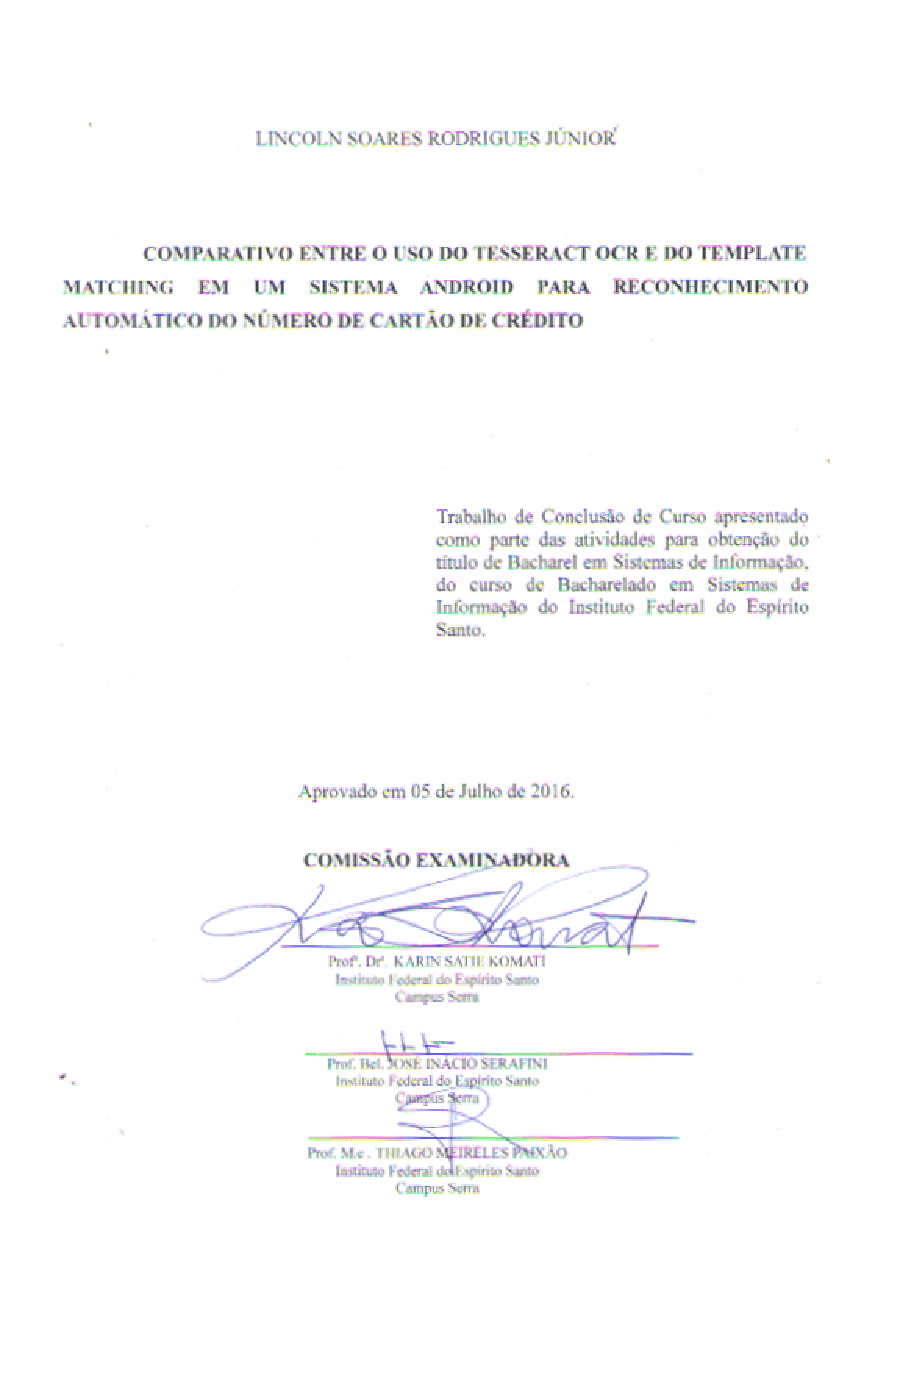
\includepdf{aprovacao.pdf}
%

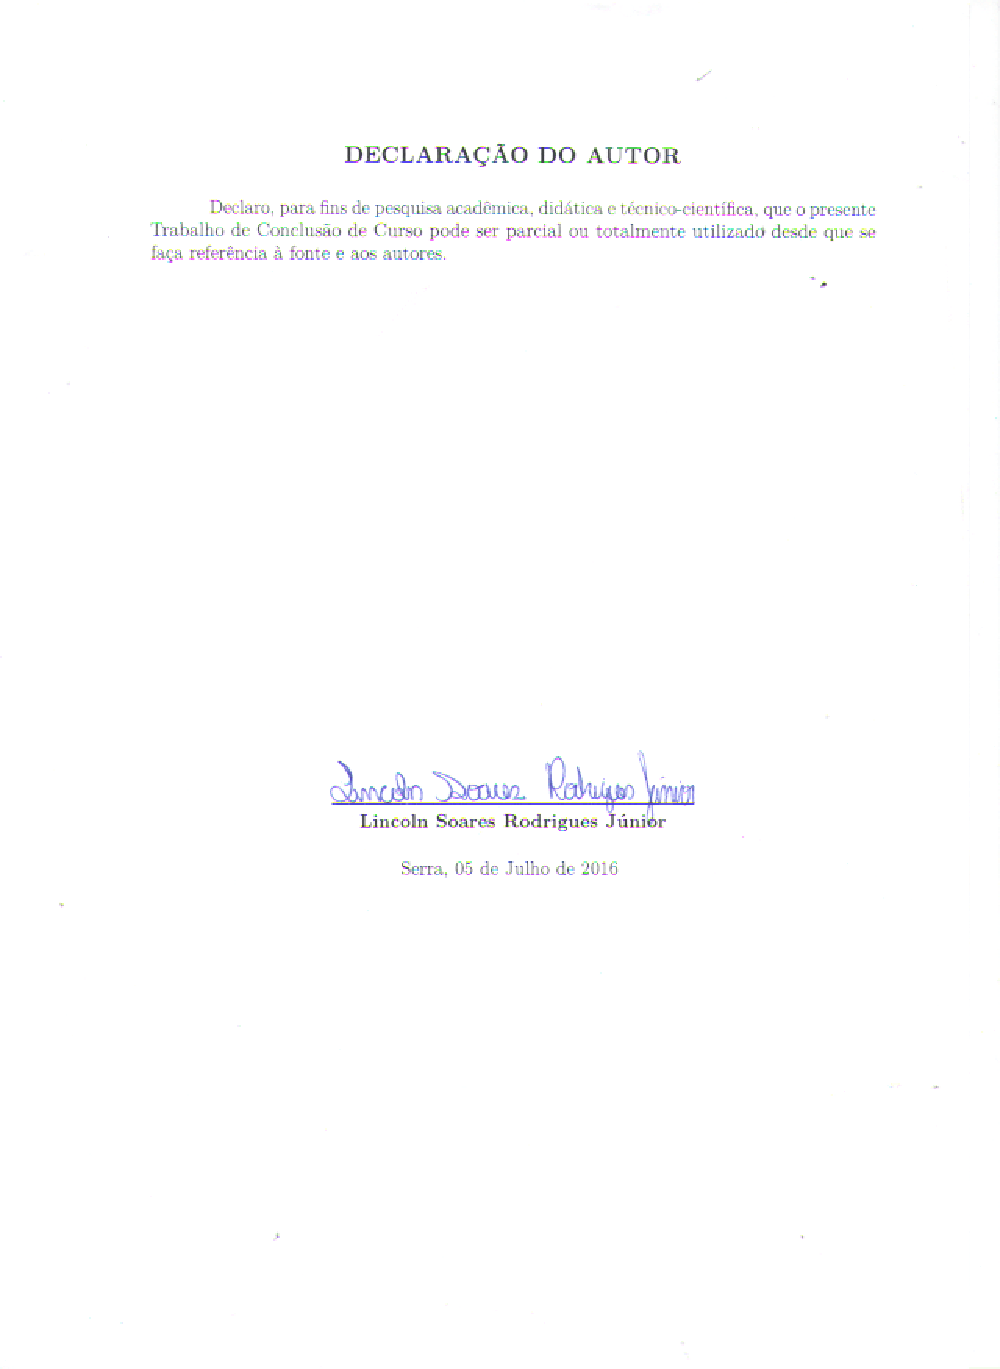
\includepdf{declaracao.pdf}

\begin{comment}
\cleardoublepage
\begin{folhadeaprovacao}




\begin{center}

    {\large\MakeUppercase\imprimirautor}

    \vspace*{\fill}\vspace*{\fill}
    \begin{center}
      {\bfseries\large\MakeUppercase\imprimirtitulo}\par
    \end{center}
    \vspace*{\fill}

    
      \hspace{.45\textwidth}
      \begin{minipage}{.5\textwidth}
       \SingleSpacing
         \imprimirpreambulo
       \end{minipage}%
       \vspace*{\fill}
    
 \begin{center}
  
  Aprovado em 05 de Julho de 2016 \\
  \end{center}  
   
   \begin{center}
  
  \bfseries\large\MakeUppercase{Comissão Examinadora}
  \end{center}
    \vspace*{\fill}

    \setlength{\ABNTEXsignwidth}{10cm}
   
   \assinatura{\textbf{\imprimirorientador} \\ Instituto Federal do Espírito Santo \\ Orientador} 
   \assinatura{\textbf{a} \\ Instituto Federal do Espírito Santo}
   \assinatura{\textbf{a} \\ Instituto Federal do Espírito Santo}

   \begin{center}
    \vspace*{0.5cm}
    {\large\imprimirlocal}
    \par
    {\large\imprimirdata}
    \vspace*{1cm}
  \end{center}
\end{center}  
\end{folhadeaprovacao}

% ---

%Declaração do Autor
\cleardoublepage
\begin{folhadeaprovacao}




  \begin{center}
  
  \bfseries\large\MakeUppercase{Declaração do Autor}
  \end{center} 
  
  Declaro, para fins de pesquisa acadêmica, didática e técnico-científica, que o presente Trabalho de Conclusão de Curso pode ser parcial ou totalmente utilizado desde que se faça referência à fonte e aos autores.

    \vspace{10 cm}
   
   \assinatura{\textbf{\imprimirautor} }    
      
   \begin{center}    
    {\imprimirlocal}, X de Julho de {\imprimirdata}
    \vspace*{1cm}
  \end{center}

\end{folhadeaprovacao}
\end{comment}}
%----

% ---
% Dedicatória
% ---
\cleardoublepage
\begin{dedicatoria}
   \vspace*{\fill}
   \centering
   \noindent
   \textit{ Aos meus pais }  \\
   \textit{ Aos xxx } \vspace*{\fill}
\end{dedicatoria}
% ---

% ---
% Agradecimentos
% ---


\cleardoublepage
\begin{agradecimentos}
Agradecimentos


\end{agradecimentos}

% ---

% ---
% Epígrafe
% ---
\begin{epigrafe}
    \vspace*{\fill}
	\begin{flushright}
		\textit{Texto motivador} \\ \\ Winston Churchill
	\end{flushright}
\end{epigrafe}


% ---

% ---
% RESUMOS
% ---

% resumo em português
\setlength{\absparsep}{18pt} % ajusta o espaçamento dos parágrafos do resumo
\begin{resumo}

Um dos grandes problemas enfrentados pelos pesquisadores é o estudo das doenças complexas, pois elas são poligênicas e multifatoriais, fazendo com que diferentes estudos apresentem baixa replicabilidade.
Recentemente, avanços significativos tem sido obtidos por métodos que realizam integração de dados entre expressão gênica e dados de rede PPI (\textit{Protein Protein Interaction Network}).
Dentre eles destaca-se o método NERI que obteve bons resultados de replicabilidade.
Esse método baseia-se nas hipóteses da \textit{Network Medicine} combinadas com métodos de importância relativa em redes complexas.
A importância relativa é uma forma de inferir a relevância topológica dos nós da rede baseado em um conjunto de nós conhecidos como sementes. Entretanto, esse método carece de uma análise de robustez, que avalie o quanto seus resultados são dependentes dos genes sementes.
Neste trabalho, analisamos a robustez do método NERI com relação aos genes sementes visando avaliar o impacto da remoção progressiva destes.
Realizamos experimentos mantendo fixos a rede PPI e os dados de expressão, 
mas removendo progressivamente parte dos nós sementes do conjunto original (de forma similar as técnicas de avaliação de classificadores \textit{leave-one-out} e validação cruzada), e comparando a interseção entre seus resultados com o resultado original.
%
Variamos o percentual de genes sementes excluídos entre 10 e 40\% e, em seguida, comparamos os primeiros elementos das listas resultantes com os primeiros da lista original.
%
Considerando o melhor cenário (remoção de 10\% das sementes), as listas resultantes apresentaram em média 90\% de interseção com a lista original, e mesmo no pior cenário (remoção de 40\% das sementes), a interseção foi de 60\% em média.
Além disso, observamos também que quanto maior a lista dos primeiros genes comparados, menor é a variância das interseções das listas resultantes com a lista original.
%
Portanto, o método NERI pode ser considerado robusto com relação aos genes sementes, indica replicabilidade mesmo em situações onde os genes sementes são variados.


Palavras chaves: Network Medicine, Validação Cruzada, Leave-one-out, Robustez.
\end{resumo}

An importante problem faced by researchers is the study of complex diseases, because they are polygenic and multifactorial, implying small replicability among different studies.
Recently, significant advances have been reached by methods that perform data integration between gene expression and PPI (Protein-Protein Interaction Network) data.
Among them, we highlight the NERI method which achieved good replicability results.
This method is based on Network Medicine hypotheses combined with relative importance analyses in complex networks.
Relative importance assesses the topological relevance of network nodes based on a set of important nodes known as seeds.
However, until this date no robustness analysis was conducted for the NERI method, in order to evaluate how much its results are dependent on the seed genes.
In this work, we analyzed the robustness of the NERI method with regard to the seed genes in order to evaluate the impact of their progressive removal.
We performed experiments fixing the PPI network and expression data, but progressively removing parts of the seed nodes from the original set (analogous to the classification assessment techniques, such as cross-validation), and comparing the intersection between their results and the original result.
We excluded between 10%--40% of the seed genes and compared the top elements of the resulting lists with the top ones from the original list.
Considering the best scenario (removal of 10% of seeds), the resulting lists averaged 90% of intersection with the original list, and even in the worst case scenario (removal of 40% of seeds), the intersection was 60% in average.
In addition, we also note that the larger the list of the first genes compared, the smaller is the variance of the intersections of the resulting lists with the original list.
Therefore, the NERI method can be considered robust with respect to the exclusion of seed genes, also presenting good replicability in such a case.
% resumo em inglês
\captionsenglish



\begin{resumo}
    
An importante problem faced by researchers is the study of complex diseases, because they are polygenic and multifactorial, implying small replicability among different studies.
Recently, significant advances have been reached by methods that perform data integration between gene expression and PPI (Protein-Protein Interaction Network) data.
Among them, we highlight the NERI method which achieved good replicability results.
This method is based on Network Medicine hypotheses combined with relative importance analyses in complex networks.
Relative importance assesses the topological relevance of network nodes based on a set of important nodes known as seeds.
However, until this date no robustness analysis was conducted for the NERI method, in order to evaluate how much its results are dependent on the seed genes.
In this work, we analyzed the robustness of the NERI method with regard to the seed genes in order to evaluate the impact of their progressive removal.
We performed experiments fixing the PPI network and expression data, but progressively removing parts of the seed nodes from the original set (analogous to the classification assessment techniques, such as cross-validation), and comparing the intersection between their results and the original result.
We excluded between 10\%--40\% of the seed genes and compared the top elements of the resulting lists with the top ones from the original list.
Considering the best scenario (removal of 10\% of seeds), the resulting lists averaged 90\% of intersection with the original list, and even in the worst case scenario (removal of 40\% of seeds), the intersection was 60\% in average.
In addition, we also note that the larger the list of the first genes compared, the smaller is the variance of the intersections of the resulting lists with the original list.
Therefore, the NERI method can be considered robust with respect to the exclusion of seed genes, also presenting good replicability in such a case.

Keywords: Network Medicine; PPI Network; Relative Importance; NERI Method; Seed Robustness.
\end{resumo}


    

\captionsbrazil
% ---

% ---
% inserir lista de ilustrações
% ---
\pdfbookmark[0]{\listfigurename}{lof}
\listoffigures*
\cleardoublepage
% ---


% ---
% inserir lista de Grafico
% ---
%\newlistof{listofgraficos}{grafico}{Lista de Gráficos}
%\renewcommand{\listgraficoname}{Gráfico}
%\renewcommand{\cftlistofgraficospresnum}{AAA~}


\begin{comment}

\end{}%\pdfbookmark[0]{\listgraficoname}{log}
\newcommand{\cftgraficopresnum}{AAA}
%\listofgraficos
\listof{grafico}{Lista de Gráficos}

\cleardoublepage
\end{comment}
% ---

% ---
% inserir lista de tabelas
% ---
\pdfbookmark[0]{\listtablename}{lot}
\listoftables*
\cleardoublepage
% ---

% ---
% inserir lista de abreviaturas e siglas
% ---
\begin{comment}


\begin{siglas}
  \item[ABNT] Associação Brasileira de Normas Técnicas
  \item[abnTeX] ABsurdas Normas para TeX
\end{siglas}
\end{comment}
% ---

% ---
% inserir lista de símbolos
% ---
\begin{comment}
\begin{simbolos}
  \item[$ \Gamma $] Letra grega Gama
  \item[$ \Lambda $] Lambda
  \item[$ \zeta $] Letra grega minúscula zeta
  \item[$ \in $] Pertence
\end{simbolos}
\end{comment}
% ---

% ---
% inserir o sumario
% ---
\pdfbookmark[0]{\contentsname}{toc}
\tableofcontents*
\cleardoublepage
% ---



% ----------------------------------------------------------
% ELEMENTOS TEXTUAIS
% ----------------------------------------------------------
\textual

% ----------------------------------------------------------
% Introdução (exemplo de capítulo sem numeração, mas presente no Sumário)
% ----------------------------------------------------------
\captionsetup[figure]{justification=justified,singlelinecheck=false}

%tabulacao para a listagem
\newcommand{\itab}[1]{\hspace{0em}\rlap{#1}}
\newcommand{\tab}[1]{\hspace{.2\textwidth}\rlap{#1}}
%inicio do capitulo
\chapter[Introdução]{Introdução}

%\textit{} // Coloca em italico
%\cite{} //Cita autor
%\ref{} //Cita figura

Doenças complexas são poligênicas e multifatoriais, ou seja, além de serem causadas por mutações em mais de um gene, também são influenciadas por fatores ambientais \cite{davey-mith}. Como título de informação, alguns exemplos de doenças complexas são doença de Parkinson e esclerose múltipla \cite{Hunter-2005}. Quanto aos fatores genéticos, devido ao fato destas doenças serem poligênicas, as mutações podem levar a uma propagação não natural de informação e sinais, de forma que afete outros genes e/ou mecanismos dependentes dos que sofreram determinada mutação. 


% \par
% \begin{figure}[ht!]
% \centering
% \includegraphics[width=150mm]{Images/pesquisaCrescimentoNumSmarth.png}
% \caption{Compras feitas através de dispositivos móveis. Imagem retirada de \cite{MarketingCharts2014}} \label{imagemDigitalCap1}
% \end{figure}


Uma forma de estudar este tipo de doença, é analisar os transcritos gerados pela transcrição dos genes, de forma a buscar uma relação de co-expressão, tendo como objetivo encontrar genes que influenciam na doença em questão. Uma forma de utilizar estes dados, é fazer a modelagem em forma de rede, onde cada nó representa um gene, as arestas representam a co-expressão genica, e ao utilizar a topologia de redes com pesos, o fator de co-expressão torna-se então o peso, determinando assim o grau de relacionamento entre dois nós, com essa abordagem, é possível aplicar conceitos e propriedades de grafos no problema, devido ao fato de ele estar modelado em rede.
Outra forma de estudar as doenças poligênicas, é analisar as interações entre proteínas (\textit{PPI – Protein-Protein Interaction}), onde também é aplicada a abordagem de redes para investigação da doença, no qual é chamada de hipótese da \textit{Network Medicine} \cite{barabasi}. Este modelo leva em conta o nível de interação entre as proteínas e quais foram os genes responsáveis por gerá-las, podendo assim ter um mapeamento gênico e proteico ao mesmo tempo.

Estas duas abordagens citadas englobam conceitos de redes complexas, onde têm-se a representação de dados e relações entre eles em forma de grafos, sejam eles com pesos ou não (em sua grande maioria são utilizados grafos direcionados e com peso), esta abordagem permite utilizar conceitos fundamentados sobre teoria de grafos e algoritmos consolidados para análise do problema, ganhando-se assim mais ferramentas para tratamento do modelo em questão.
Como por exemplo, algoritmos de caminho mínimo, onde visam encontrar o menor caminho entre dois nós, na genética, cada aresta é uma relação entre os genes (\textit{nós}), portanto, quanto o menor caminho entre dois genes (\textit{nós}), mais próxima é a sua relação. 

De acordo com os conceitos apresentados, existem diversas abordagens para tratar doenças poligênicas, dentre elas, destaca-se o método NERI que apresentou bons resultados de replicabilidade. Este é um método que baseia-se em importância relativa, ou seja, fundamenta-se em nós sementes para o seu funcionamento, onde estes são genes sabidamente reconhecidos como importantes. Em vista desta abordagem, este método carece de uma análise de robustez, o que significa analisar o quão dependente dos nós sementes o método é, de forma a encontrar um coeficiente de confiança, para assim gerar uma segurança na utilização da ferramenta, porém, para encontrar estes coeficientes é necessário observar o comportamento do método quando há retiradas de nós sementes da rede de entrada.

Ao analisar o código fonte do programa em questão, identificamos a necessidade de reestruturação do mesmo, de forma que fique mais modularizado, facilitando a manutenção e adição de novas funcionalidades futuras, também temos como objetivo facilitar e incentivar a colaboração de pesquisadores no desenvolvimento futuro da ferramenta, pelo fato de o código ser aberto, ou seja, qualquer um que estiver disposto a contribuir terá acesso ao código fonte.
Como a ferramenta foi desenvolvida para ser utilizada por biólogos, identificamos também, a necessidade de desenvolver uma interface gráfica para facilitar e disseminar o uso. Atualmente a utilização é feita somente por linha de comando no terminal, o que requer um nível de conhecimento mínimo. A interface gráfica tem como objetivo viabilizar o uso do programa para biólogos não familiarizados em utilizar programas por linhas de comando em terminal, potencializando assim o alcance da ferramenta e incentivando o uso de métodos computacionais por biólogos.


%Exemplo de imagem

%\textbf{\begin{figure}[ht!]
%\centering
%\includegraphics[width=130mm]{Images/debit.jpg}
%\caption {A evolução das máquinas de cartão. \label{adas}}
%\flushleft{Fonte: Imagem de retirada e adaptada de \cite{evolu}.}
%\end{figure}}

%\begin{figure}[ht!]
%\centering
%\includegraphics[width=130mm]{Images/debit.jpg}
%\caption {A evolução das máquinas de cartão. \label{Evolucao}}
%\flushleft{Fonte: Imagem de retirada e adaptada de \cite{evolu}.}
%\end{figure}


%\section{OCR} // Criando sessao



\section{Objetivos}
\subsection{Objetivo Geral}
\begin{center}
  \begin{enumerate}
  \item {Analisar robustez do método NERI para avaliar o impacto da retirada de alguns genes sementes.}

  \end{enumerate}
\end{center}

\subsection{Objetivos Específicos}
\begin{center}
  \begin{enumerate}
  \item {Refatorar o código para facilitar a manutenção, utilização e contribuição externa da comunidade de usuários e desenvolvedores.}
    \item {Implementar os algoritmos de validação cruzada e \textit{leave-one-out} aplicados ao método NERI.}
    \item{Implementar interface gráfica para facilitar o uso da ferramenta, visando torná-la mais intuitiva e amigável aos pesquisadores da área biológica.}
  \item{Desenvolver um módulo de \textit{Template Matching}.}
    \item {Analisar a robustez do método NERI verificando sua dependência em relação aos nós sementes.}
  \end{enumerate}
\end{center}


\section{Organização do trabalho}
Escrever


% ----------------------------------------------------------
% PARTE
% ----------------------------------------------------------
%\part{Preparação da pesquisa}
% ----------------------------------------------------------

% ----------------------------------------------------------
% PARTE
% ----------------------------------------------------------
%\part{Referenciais teóricos}
% ----------------------------------------------------------

% ---
% Capitulo de revisão de literatura
% ---
\chapter{Referencial Teórico}

\index{Referencial Teórico }
	 
% \section{Fundamentos Teóricos}
\par
    Para melhor compreensão do conteúdo apresentado neste trabalho, este capítulo tem como objetivo explicar os fundamentos conceituais necessários para garantir a boa compreensão e evolução do conteúdo.
    
\section{Fundamentos Matemáticos}

\subsection{Grafos}
Grafos são formas de estruturação de dados ligados pertencentes ao mesmo conjunto. Um elemento recebe a denominação de nó ou vértice. As relações entre os nós são definidas por \textit{arestas}.
Para exemplificação, tome como nós, cidades \textit{n1},\textit{n2}, \textit{n3} e \textit{n4}, onde as estradas que fazem conexão entre estas cidades representam as arestas \ref{graph_base}. Com este conceito, pode-se modelar estas ligações em forma de grafo. \cite{Graph_teory}
%
%Imagem
\begin{figure}[ht!]
\centering
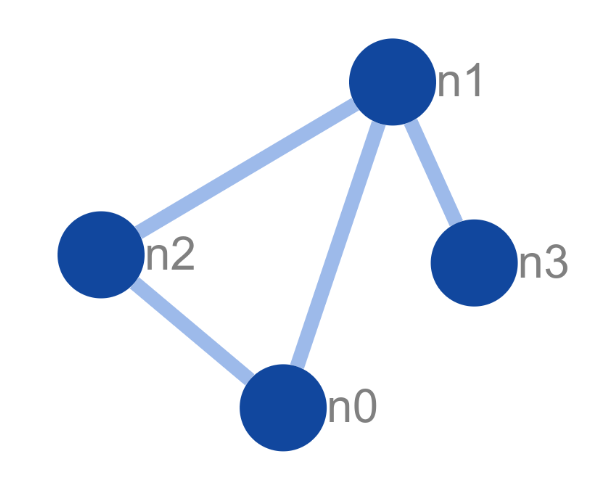
\includegraphics[width=50mm]{Images/graph_base.png}
\caption {Representação em grafo
\label{graph_base}}
\flushleft{Fonte: Produzido pelos autores.}
\end{figure}


\subsection{Grafos com pesos}
São grafos que possuem um \textbf{grau de importância} (também chamado de peso) em cada \textbf{aresta}, este \textbf{grau de importância} tem significado apenas em nível de abstração, ou seja, não carrega uma interpretação predefinida. Geralmente, exprime o quão \textbf{relacionado} um nó está com outro, onde esta informação é interpretada de acordo com o contexto no qual está inserido.\cite{Graph_teory}

Figura representativa~\ref{graph_wheigth}.
%
%Imagem
\begin{figure}[ht!]
\centering
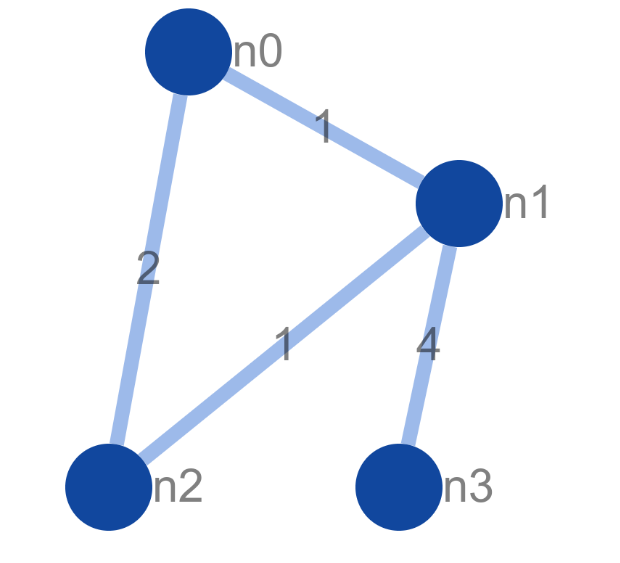
\includegraphics[width=50mm]{Images/graph_wheigth.png}
\caption {Grafo com peso
\label{graph_wheigth}}
\flushleft{Fonte: Produzido pelos autores.}
\end{figure}

\subsection{Passeio}
É uma sequência específica de nós ligados, partindo de \textbf{\textit{p}} e chegando em \textbf{\textit{g}} \cite{Pavlopoulos2011}. Onde o \textbf{comprimento} do \textit{passeio} é determinado pelo número de \textit{arestas} percorridas.
%
Tomando o \textsl{grafo} representado pela Figura~\ref{graph_path}, um dos \textbf{passeios} possíveis de \textsl{p} a \textsl{q} é o conjunto \textsl{A}, formado pelos nós visitados \textit{A =\{p,r,t,v,t,q\}}. O \textbf{comprimento do passeio} \textsl{A} é \textit{6}, como também pode ser definido como o tamanho do \textit{conjunto} de nós visitados \textit{menos 1}.
%
%Imagem
\begin{figure}[ht!]
\centering
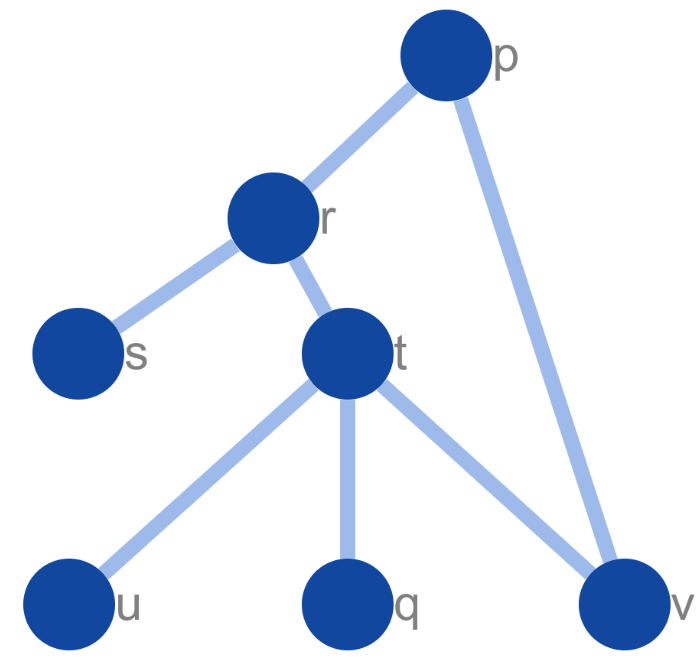
\includegraphics[width=50mm]{Images/graph_path.png}
\caption {Grafo
\label{graph_path}}
\flushleft{Fonte: Produzido pelos autores.}
\end{figure}


\subsection{Caminho e distância}
Assim como o \textit{passeio}, o \textit{caminho} é uma sequência específica de nós ligados. Porém este não possui vértices repetidos, ou seja, não passa duas vezes pelo mesmo vértice \cite{Pavlopoulos2011}. 
Se tomarmos como exemplo o grafo da imagem \ref{graph_path}, um \textbf{caminho} de \textit{p} a \textit{q} é a sequencia de nós \textit{\{p,r,t,q\}}. 
A \textbf{distância} do \textit{caminho} é definida pela soma dos pesos em suas arestas em \textit{grafos com pesos}. Para os \textit{grafos sem peso}, a \textbf{distância} é definida pela quantidade de arestas presentes no \textit{caminho}, implicitamente definindo o peso de cada \textit{aresta} como \textit{1} e executando a soma das mesmas.
No \textbf{caminho} \textit{\{p,r,t,q\}} a \textbf{distância} entre \textit{p} e \textit{q} é \textit{4}.


%\subsection{Distância}
%Em grafos com peso, é definida pela soma dos pesos das arestas em um determinado caminho.
%Em grafos sem peso, é definida como a quantidade de arestas (aresta peso 1) em um determinado %caminho.

%Imagem


\subsection{Nó Hub}
Hub é um nó que possui muitas arestas, ou seja, um nó que se liga a muitos outros nós \cite{Pavlopoulos2011}.
Na imagem \ref{graph_hub} o \textsl{hub} é o nó \textsl{t}, ou seja, é o nó que possui mais arestas \textsl{6} do grafo.
%
%Imagem - HUB
\begin{figure}[ht!]
\centering
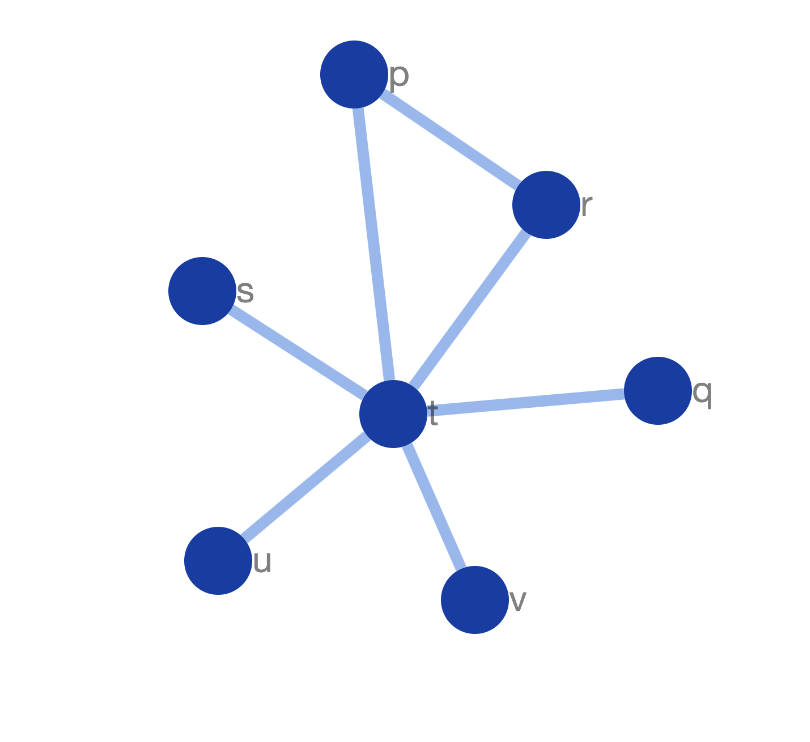
\includegraphics[width=80mm]{Images/graph_hub.png}
\caption {Representação de \textsl{Hub}
\label{graph_hub}}
\flushleft{Fonte: Produzido pelos autores.}
\end{figure}


\subsection{Nó Bridge}
Nós \textsl{bridge} ou ponte são nós que conectam duas comunidades ou módulos de rede, ou seja, é uma medida que determina o quanto um nó liga dois grandes agrupamentos \cite{Hwang2006}.
Na Figura~\ref{graph_bridge} o nó \textbf{\textsl{n16}} é um definido como \textsl{bridge} e os nós \textbf{\textsl{t}} e \textbf{\textsl{n13}} são \textsl{Hubs}, mesmo o nó \textsl{\textbf{n16}} não estando diretamente ligado nos nós \textsl{Hubs}, ele apresenta o comportamento de \textsl{Bridge} por estar conectando os dois grandes agrupamentos.
%
%Imagem - BRIGDE
\begin{figure}[ht!]
\centering
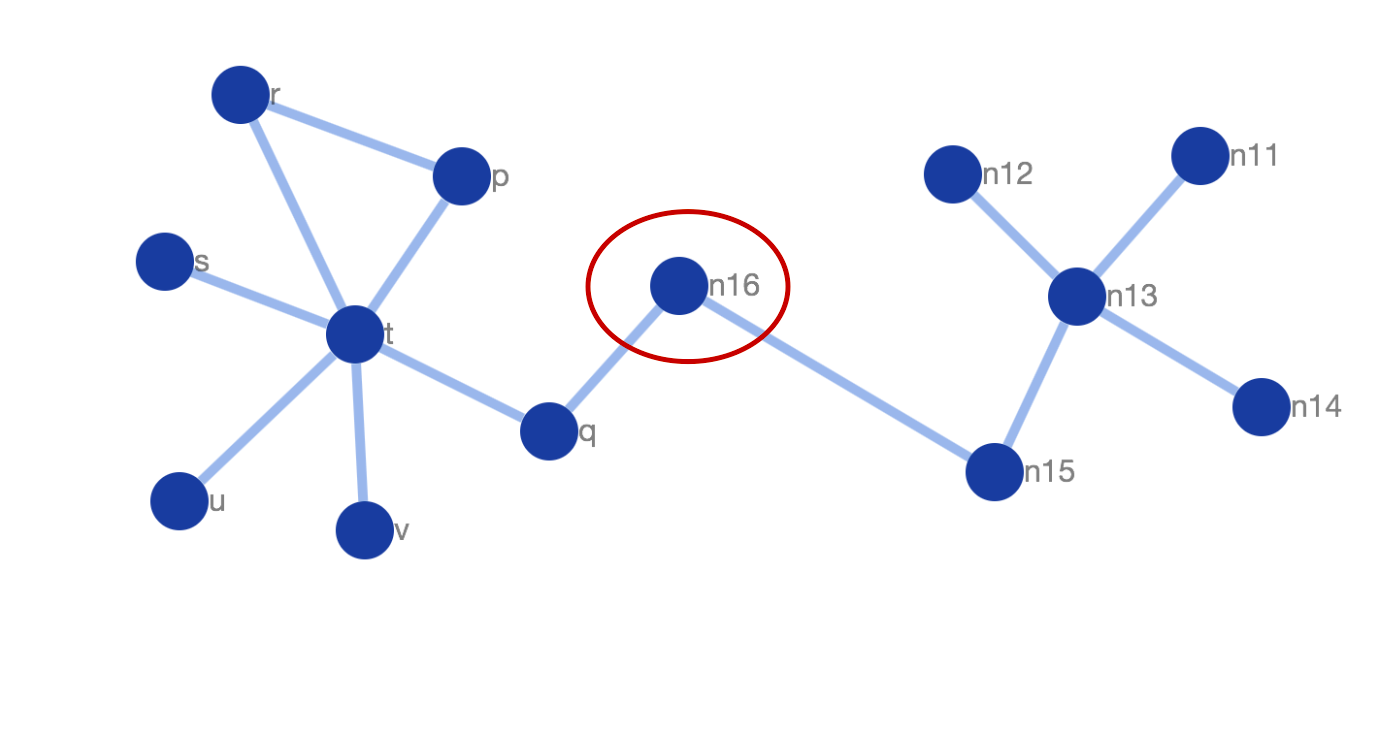
\includegraphics[width=\textwidth]{Images/graph_bridge.png}
\caption {Representação de um nó \textsl{bridge}
\label{graph_bridge}}
\flushleft{Fonte: Produzido pelos autores.}
\end{figure}

\subsection{Menor caminho ou caminho mínimo}
Quando se trata de grafos o \textbf{caminho mínimo} é aquele que possui a menor distância entre dois nós (\textsl{p} e \textsl{g}) \cite{Dijkstra1959}. No grafo com pesos representado pela Figura~\ref{graph_wheigth}, o caminho mínimo entre os nós \textsl{n2} e \textsl{n3} é dado pelo conjunto de nós \textsl{\{n2,n1,n3\}}, sendo a distância entre \textsl{n2} e \textsl{n3} igual a \textsl{5}. Um outro caminho válido mas que não é mínimo entre \textsl{n2} e \textsl{n3} é dado pelo conjunto de nós conectados \textsl{\{n2,n0,n1,n3\}}, no qual a distância entre \textsl{n2} e \textsl{n3} é igual a \textsl{7}. Ambos são caminhos válidos no mesmo grafo, porém o menor caminho possível entre \textsl{n2} e \textsl{n3} neste grafo é \textsl{\{n2,n1,n3\}}.
%Imagem

\subsection{Redes complexas}

O estudo de redes complexas é uma área relativamente recente e ativa da pesquisa científica e foi inspirada em grande parte pelo estudo empírico de redes do mundo real, como redes de computadores, redes tecnológicas, redes cerebrais e redes sociais.
Uma rede complexa pode ser representada por um grafo características topológicas não triviais, ou seja, 
características que não ocorrem em redes simples tais como reticulados, e nem ocorrem em gráficos aleatórios, mas geralmente ocorrem em modelos de sistemas reais.

O conceito de redes complexas é muito importante para representação de sistemas complexos, sendo que os mesmos podem ser representados em forma de grafos e consequentemente em rede \cite{Strogatz2001}. Porém, redes complexas devem apresentar estruturas topológicas não triviais, ou seja, possuírem um conjunto de vértices que sejam interconectados por arestas \cite{Barabasi2003}.
%

Uma característica importante das redes complexas, são as suas propriedades, como por exemplo, as medidas de centralidade que apontam comportamentos de um determinado nó ou um conjunto deles. Isto faz com que a análise destes dados representem algo direto no problema, visto que a rede é uma abstração do problema real \cite{Metz2007}.
Tais características auxiliam na abstração do problema, onde o pesquisador interpreta cada comportamento encontrado na rede, uma aplicação no "\textsl{mundo real}" estudado.
%
Ao permitir que um problema seja modelado e representado por uma rede complexa, pode-se estudá-la utilizando os ferramentais desenvolvidos para grafos e redes complexas. Isto auxilia a resolução do problema, pois permite ao pesquisador utilizar conceitos já validados. 	

% ===================== FUNDAMENTOS BIOLÓGICOS ========================== 

\section{Fundamentos biológicos}

%\subsection{Dogma central da biologia}

%\textcolor{red}{Conceito de transcrição e fundamento da genômica ACHO IMPORTANTE ABORDAR}

%imagem

\subsection{Co-expressão de transcritos}

A correlação de duas variáveis significa o quanto o comportamento de ambas está relacionado, ou seja, se a variação de uma variável \textsl{A} acompanha a variação da variável \textsl{B}. Este fator funciona tanto para variações diretamente proporcionais quanto para variáveis inversamente proporcionais, sendo as diretamente proporcionais quando as duas variáveis possuem variações de mesmo sinal e a inversamente proporcional quando as variações são em relação a sinais opostos.
De forma mais objetiva, correlação é uma medida que varia de -1 a 1, onde representando o valor -1 as variáveis analisadas são inversamente proporcionais, ou seja, quando o valor uma variável aumentou as outras diminuíram e vice versa. Quando o fator é 0 as variáveis não tem relação nenhuma, significando que há variação em uma ou mais variáveis, não necessariamente há variação nas outras. E por fim, quando o se apresenta com o valor 1, significa que as variáveis em questão variam juntas, onde quando há aumento do valor de uma ou mais variáveis, todas as outras também apresentaram um aumento em seus valores, o mesmo comportamento se mantém se houver a diminuição do valor em uma ou mais variável, todas as outras irão acompanhar apresentando diminuição nos seus respectivos valores.

O conceito de co-expressão é a correlação de transcritos gênicos, onde determina-se o quanto a variação de um gene está relacionado com outro. Definindo, desta forma valores de co-expressão transcriptômica entre os genes
\cite{Gaiteri2014}.



% ADICIONAR REFERENCIA

%\subsection{Doenças poligênicas e multifatoriais}
%Representam um fenótipo ou determinam a doença.
%O que significa, a doença não é composta por um único pedaço de DNA sequenciado, mas sim por vários pedaços de locais separados. \cite{barabasi}

%O fato da mesma ser multifatorial, implica não somente aos pedaços de DNA envolvidos mas também aos fatores externos em que o indivíduo está submetido. Este aspecto torna ainda mais complexo o estudo deste tipo de doenças.

%São doenças que não possuem um unico gene causador ou impactante, são afetadas por mais de um fator de ativação, desta forma a complexidade do estudo das mesmas aumenta

%Imagem


\section{Rede PPI}

Redes PPI (Protein-protein Interaction), são redes que representam dados de interação entre diferentes proteínas que indicam como as mesmas ativam ou não processos biológicos dentro das células \cite{Pavlopoulos2011}.
Apesar das interações entre diferentes proteínas e suas respectivas sequencias gênicas estarem praticamente todas descobertas, ainda não se sabe completamente suas funções moleculares.
Através da modelagem das interações em rede, é possível inferir funções proteicas com a interação entre outras biomoléculas.
%

Assim como as interações entre proteínas podem ser mapeadas em rede, surge um novo conceito denominada \textsl{Network Medicine} por \cite{Barabasi2011}, onde o autor aborda doenças humanas mapeando-as em redes complexas. Desta forma, pode-se estudar não só os fatores de complexidade molecular relacionados a uma determinada doença, mas também é possível analisar os fenótipos relacionados, levando à possibilidade de encontrar uma via biológica relacionada a doença.

\section{Redes Biológicas}

%\subsection{Representação de genes em rede}
%\textcolor{red}{=== Texto ===}

%\textcolor{red}{=== ORGANIZAR E FALAR UM POUCO DE CADA UM DESTES TRABALHOS ===}
%	Using graph theory to analyze biological networks
%	\cite{Pavlopoulos2011}
%	An Integrative Systems Medicine Approach to Mapping Human Metabolic Diseases
%	\cite{Barabasi2011}
%	Exploring the human diseasome: The human disease network 
%	\cite{Goh2012}
%	Network Medicine
%	\cite{Barabasi2003}	
%	Neste trabalho é definido o conceito de Network Medicine, este no qual baseia-se o método NERI.
%<Descrever artigo>



\subsection{Relação de menor caminho}

A relação de menor caminho em uma rede biológica determina o quão próximo dois elementos estão do outro, sendo assim uma possível via biológica de interferência direta de um elemento a outro. Como por exemplo na rede gênica, o caminho entre os genes pode ser entendido como uma via biológica de ativação, apresentando um ponto para estudo e validação por um pesquisador.

\subsection{Redes de Co-expressão}
As redes podem ser representadas como grafos sem peso e grafos com peso. No caso das redes que utilizam dados de co-expressão, os valores encontrados são utilizados como pesos entre os genes em representados na rede. Isto se aplica pelo fato do peso entre dois nós representar o quão relacionados eles estão. Neste mesmo contexto, os dados de co-expressão determinam o quanto a transcrição de um gene está relacionada coma transcrição de outro gene. Por este motivo, mapeia-se os valores de co-expressão entre os genes para os pesos relativos na rede, determinando o grau de proximidade entre eles com valores reais obtidos por análise \cite{Gaiteri2014}.

%\subsection{Conceito de genes e nós sementes }
%\textcolor{red}{=== Texto ===}

\subsection{Importância relativa}

Em grafos grandes e complexos, as relações entre os nós e suas conexões geralmente exprimem um significado. O estudo destas relações é importante para análise dos dados que o grafo representa, assim sendo,
surge a necessidade de identificar quais são os nós mais importantes da rede em relação aos nós sementes. A necessidade de determinar esta importância é denominada \textsl{Importância Relativa}. 
%

Este é um tema que gerou publicações importantes no estudo de redes complexas. Um destes estudos é do \cite{White2003}, que propuseram diferentes maneiras de eleger os nós mais importantes de uma rede. Assim como a pesquisa no qual este trabalho propõe a validação o \cite{Simoes2015}, utiliza destes conceitos para eleger os genes mais importantes relacionados a doença em estudo.
%

Importância relativa é essencial na abordagem de redes complexas, devido ao fato de elencar os nós mais importantes baseados em um conhecimento prévio. Este conhecimento prévio é modelado em nós sementes, ou seja, alguns nós que previamente são conhecidos por sua importância, são utilizados como ponto de partida e elementos chaves para a busca de outros nós importantes na rede. Este estudo baseia-se na importância relativa individual, ou seja, a importância de um nó em relação ao conjunto.

%Assim sendo, dado um grafo \textsl{G(N,A)} e o conjunto ${{S} \in {N}}$  sendo os nós sementes, para calcular a importância relativa de um nó ${{p} \in {N}}$ em relação ao conjunto \textsl{S} é dada pela equação na Figura~\ref{ir_function}.

%
%Imagem - calculo
%\begin{figure}[ht!]
%\centering
%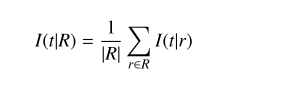
\includegraphics[width=50mm]{Images/ir_function.png}
%\caption {Equação de importância relativa
%\label{ir_function}}
%\flushleft{Fonte: Produzido pelos autores.}
%\end{figure}


%
%%$I = {{A \cup B} \over |A|}$
% EQUAÇÂO (2.7 -> NERY)
%

Outro modelo de importância relativa é a definição dos caminhos mais importantes na rede, ou seja, o melhor caminho entre em dado nó \textsl{p} ao nó \textsl{q}. Este conceito também é aplicado pelo \textsl{Método NERI}, onde os caminhos são identificados como vias biológicas da doença em estudo. Este conceito se popularizou com o \cite{Barabasi2011} denominado \textsl{Network Medicine}, abrindo caminho para diversas pesquisas na área e criando um conceito novo de estudo para doenças complexas e multifatoriais.
%

Um ponto que deve ser ressaltado é no \textsl{Método NERI}, onde o autor aplica dois escores para priorização gênica. Estes escores são utilizados como fator de ranqueamento dos genes mais influentes para uma determinada doença, são eles $\Delta'$ e $X$. O score de ranqueamento baseado em importância relativa $\Delta'$, que prioriza a maior alteração entre as pontuações em cada condição, e o score $X$ que privilegia a maior soma das pontuações definidas. Estes scores são responsáveis por selecionar os genes mais relacionados a doença estudada.

% ==== ANÁLISE DE ROBUSTEZ ====

\section{Análise de robustez}

\subsection{Método K-Fold Cross-Validation}


O método \textsl{K-Fold Cross-Validation}, também chamado de estimativa de rotação, é uma técnica desenvolvida para avaliar a capacidade de generalização de um determinado modelo em relação a um conjunto de dados. Este modelo analisa os resultados estatísticos de um agrupamento de dados definido, onde tem sido amplamente empregado em problemas no qual o objetivo da modelagem é  predição de dados, isto se dá por seu conceito principal consistir no particionamento dos dados de entrada em subconjuntos mutualmente exclusivos, onde uma parte destes serão revezados na alimentação do modelo a ser validado (grupo de treinamento), e a outra parte utilizados na validação.
%

Esta separação é feita de forma que o um conjunto seja divido \textsl{K} subconjuntos de tamanhos iguais ou quase iguais. Após a criação dos \textsl{K} conjuntos, o modelo em questão, é treinado com \textsl{K - 1} conjuntos. De forma que o conjunto que sobrou seja utilizado como teste dos resultados gerados pela etapa de treinamento. Comumente, os dados presentes nos conjuntos são estratificados para que cada subconjunto represente da melhor forma possível o conjunto total \cite{Mudry2011}. 
%

\subsection{Método Leave-one-out Cross-Validation}

O método \textsl{Leave-one-out Cross-Validation} é um caso especial do \textsl{K-Fold Cross-Validation}, onde a quantidade de subconjuntos gerados é do tamanho do conjunto total de dados. O conjunto de dados original é separado de forma que cada subconjunto esteja faltando um elemento, ou seja, dado um conjunto \textsl{P} de tamanho \textsl{K}, devem ser gerados \textsl{K} subconjuntos de tamanho \textsl{K - 1}, onde todos os subconjuntos devem ser diferentes.
%

Após a separação dos subconjuntos, uma única execução do modelo é feita, assim pode-se analisar resultado daquele elemento faltante. Este modelo geralmente é aplicado em situações onde o volume de dados não é muito significante, uma área que utiliza bastante este método é a \textsl{Bioinformática}, onde poucos dados da amostra estão presentes \cite{Mudry2011}. 


\subsection{Método Repeated K-Fold Cross-Validation}

É uma variação do modelo \textsl{K-Fold Cross-Validation}, onde o objetivo é executar várias vezes os subconjuntos gerados na etapa de separação de dados visando um resultado mais confiável \cite{Mudry2011}. Assim sendo, surgem variações deste conceito, neste trabalho, mais especificamente, no Capítulo 3 apresentamos uma variação baseada neste método para análise da robustez do \textsl{Método NERI}.




% ==== FUNDAMENTOS ESTATÍSTICOS --> PROVAVELMENTE VAI SAIR

%\section{Fundamentos estatísticos}
%\subsection{Mediana}
%\subsection{Percentil}
%\subsection{Outlier}
%\subsection{Gráfico Boxplot}

% ==== TRABALHOS CORRELATOS ====

\section{Método NERI}

Para entender doenças complexas, é necessário encontrar os genes que se relacionam com a mesma.
Com a evolução em larga escala das tecnologias de sequenciamento do genoma e das medições de transcritos, assim como o conhecimento da interação presente entre proteína-proteína (PPI – \textsl{Protein Protein Interaction}), a pesquisa sobre doenças complexas vêm se tornando cada vez mais comum.
Ao basear-se no paradigma do \textsl{Network Medicine}, as redes de interação proteína-proteína têm sido utilizadas para enfatizar os genes relacionados à doenças complexas levando em conta fatores topológicos. 

O método NERI \cite{Simoes2015} procurou resolver o problema da replicabilidade através da integração de dados biológicos e as hipóteses da \textsl{Network Medicine}.
Neste projeto, analisamos a robustez deste método com relação aos genes sementes.
%
Porém este método é afetado diretamente pela literatura disponível, onde proteínas mais estudadas tendem a ter mais conexões na rede, fazendo com que diminua a qualidade dos resultados. Sendo assim, métodos que utilizam somente redes PPI não fornecem dados dinâmicos e específicos, dado que a topologia da rede não é exclusiva para uma única doença. No trabalho em questão, foi desenvolvido um método que prioriza genes e vias biológicas relacionados a uma dada doença complexa, através da abordagem de não somente redes PPI mas também transcrissômica e genômica, sendo os dados integrados em uma única rede. Após a integração e construção da rede, aplicou-se o conceito da \textsl{Network Medicine}, encontrando caminhos mínimos que possuam maior co-expressão entre seus genes. Com este modelo foi desenvolvido dois escores de ranqueamento, onde um prioriza genes com maior alteração entre suas pontuações em cada condição, e o outro privilegia os genes com a maior soma destas pontuações. Desta forma a aplicação do método em a três estudos envolvendo de expressão da doença esquizofrenia, recuperou com sucesso genes diferencialmente co-expressos em duas condições diferentes, e juntamente evitou os erros de literatura presentes na rede PPI. Em paralelo, melhorou substancialmente a replicação de resultados pelo método aplicado aos três estudos, onde por métodos convencionais, não atingiam uma replicabilidade satisfatória.




% ---
\chapter[Metodologia]{Metodologia}

Para análise de robustez do método NERI foram utilizados conceitos de validação baseados na alteração dos parâmetros de entrada, de forma que sejam analisados os resultados de saída, para entender o impacto causado devido a estas alterações, no qual consistem na remoção ou não inserção de elementos chaves para o input do programa. 

O processo de validação foi separado em etapas para melhor entendimento e apresentar a temporalidade e cadenciamento dos processos.

\section{Materiais}

Este trabalho utilizou a base de dados <BASE DE DADOS AQUI> que consiste em expressões gênicas de pessoas portadoras da doença <ESQUIZOFRENIA>, estes dados podem ser encontrados <AQUI>. Esta base de dados em específico, foi selecionada esta base devido ao fato de ter sido utilizada na tese de doutorado no qual este trabalho se baseia e se referencia, assim os dados obtidos podem ser comparados com os encontrados e apresentados pelo autor, desta forma evitando o enviesamento do resultado por diferença de experimentação.

O programa NERI também recebe dados de rede de integração proteína proteína (Protein Protein Interaction – PPI), onde os mesmos também foram mantidos os originais utilizados pelo autor, podendo ser encontradas <AQUI>.

Como entrada do sistema também são definidos os Genes Sementes, onde estes são os genes onde há certeza da sua relação com a doença analisada em questão, a base de dados original pode ser encontrada <AQUI>. 


\section{Escolha da variação dos genes sementes}
Neste trabalho, os genes sementes foram escolhidos para variação como parâmetro de entrada, onde o objetivo é identificar o impacto gerado na rede de correlação gênica e no resultado final exibido pelo programa NERI, assim podendo calcular a dependência e sensibilidade do método em relação a qualidade e quantidade de dados dos nós sementes.


\section{Escolha dos métodos de validação}
Os métodos de validação adotados foram selecionados pelas suas caraterísticas de estudo do problema em questão, não podendo deixar margem para enviesamento dos resultados e serem capazes de explorar comportamentos diferentes nos resultados do experimento. Os modelos de validação escolhidos foram: \textit{Leave one Out} e \textit{Cross Validation}.


\subsection{Leave one out}
<VERIFICAR SE FICA  AQUI MESMO>
Leave one out foi aplicado no agrupamento de genes sementes, onde cada execução do programa está faltando um gene semente diferente, de forma que sempre haja a mesma quantidade de genes em cada execução e garantindo que todos tenham ficado de fora pelo menos uma vez, assim sendo, o número final de execuções e amostras de entrada sejam a quantidade total de genes sementes menos 1 (N – 1 | N = total de genes).

Com este método, é possível descobrir, se a falta de um único gene semente é responsável por alterar significantemente o resultado final do método NERI. Desta forma, podendo analisar se o método em questão é sensível a retiradas de nós sementes. 
O Leave one Out também permite a análise de importância relativa dos genes sementes, onde aquele que causar maior impacto no resultado final indica uma importância relativa maior em relação aos outros. 


Porém há outra análise importante que deve ser feita mas o Leave One Out não é capaz de prover, é se a quantidade de nós removidos influenciam diretamente no resultado. Para observar este aspecto, utilizamos o método Cross Validation, no qual, suas características se moldam mais a esta ótica de estudo.


\subsection{Cross Validation}

Este método foi adotado pela sua característica principal, organização de agrupamentos de dados de entrada. Com esta característica chave, buscou-se estudar o comportamento da rede quando há a remoção de mais de um gene semente do agrupamento original de entrada.

Com a formação de agrupamentos de genes sementes aleatórios e de tamanhos variados, pôde-se observar o comportamento do método analisado em situações variadas, buscando o ponto de ruptura de proximidade ao resultado original, assim estimando um grau de dependência e sensibilidade a uma quantidade ou arranjo de genes sementes como parâmetro de entrada.

O fato de os agrupamentos possuírem arranjos de genes diferentes, abre-se a possibilidade de estudo sobre a eficácia de um ou mais genes semente juntos sobre o resultado final, ou seja, se um arranjo específico promove melhores resultados que os demais, sendo estes de mesmo tamanho.

\section{Preparação dos experimentos}

Após determinado os métodos de validação e a base de dados a ser aplicada para análise da ferramenta, o próximo passo é a preparação do experimento a ser desenvolvido, no caso, como a base dados utilizada apresenta 38 genes sementes, a regulação dos parâmetros de remoção para preparação do experimento deve levar em conta diretamente esta quantidade.

Os genes em questão são:
<TABELA DE GENES AQUI>

Estes dados são os brutos de entrada, como o método NERI faz a integração gênica com o GWAS, alguns destes genes, apresentados na tabela acima, não tem representação e ficam de fora, resultando em 30 genes de entrada.

Os genes resultantes são
<TABELA DOS 30 GENES AQUI>

\subsection{Aplicação do método Leave one out}

Para a validação utilizando o método Leave One Out, a preparação do experimento consistiu em gerar entradas para o NERI de forma que cada amostra de entrada tenha um gene a menos do experimento original, onde exista uma entrada para cada gene removido, ou seja, em uma amostra de 38 genes de entrada, temos 37 combinações de entradas possíveis. 
Assim sendo, dado um conjunto de N elementos, a quantidade de entradas possíveis é N-1.

<IMAGEM REPRESENTATIVA>

A aplicação direta no sistema consistem em cada execução independente do programa, o agrupamento de dados de entrada faltar um gene semente diferente, de forma que sempre haja a mesma quantidade de genes em cada execução e garantindo que todos os genes tenham ficado de fora pelo menos uma vez no total de execuções independentes.

<Para preparação destas entradas, foi desenvolvido um script em Python 3.X para automatização do processo e para evitar falha humana.>

<Script Python GERA_LOO>

Para ilustração do experimento, segue o exemplo abaixo:
Temos a amostra original A sendo: 1,2,3,4,5
Os subconjuntos gerados utilizando o conceito de Leave One Out são:
As1: 2,3,4,5
As2: 1,3,4,5
As3: 1,2,4,5
As4: 1,2,3,4

<IMAGEM ToyExampleLOO1>

\subsection{Aplicação do método Cross Validation}

Para melhor aproveitamento do método escolhido, o primeiro passo a ser dado, é a definição de tamanho dos agrupamentos de dados de entrada para cada bateria de execuções.
Levando em consideração a quantidade de genes de entrada total do experimento, 30 após a integração com o GWAS, definiu-se que as remoções seriam feitas em relação a porcentagem da amostra original, sendo as porcentagens definidas 10\% (3 genes), 20\% (6 genes), 30\% (9 genes) e 40\% (12 genes).

Com as porcentagens de remoção definidos, determinou-se a quantidade de agrupamentos de dados de entrada a serem executados para cada etapa, onde estão descritos na tabela abaixo

<COLOCAR EM TABELA>
10\% --- 50 execuções
20\% --- 50 execuções
30\% --- 50 execuções
40\% --- 50 execuções

Cada agrupamento deve ser diferente do outro, de forma que o conjunto de genes removidos não se repita dentro de cada etapa, em vista que, caso isso aconteça, a análise final será comprometida por possuir resultados iguais provenientes de entradas de dados iguais.

<Para garantir a diferença entre os dados de entrada, foi desenvolvido um script em Python 3.x para automatização da tarefa evitando falha humana no processo.>
<Script GERA_CVV>

Para ilustração do experimento, segue o exemplo abaixo:

Temos a amostra original A, sendo: 0,1,2,3,4,5,6,7,8,9.
Determinado o fator de remoção em 20%, e a quantidade de dados de entrada em 5.
Dado 20% de 10 elementos, temos fator de remoção = 2 elementos.
Temos os subconjuntos:
As1 = 0,1,2,3,4,5,6,7
As2 = 0,1,2,3,4,5,6,8
As3 = 0,1,2,3,4,5,6,9
As4 = 1,2,3,4,5,6,7,8
As5 = 2,3,4,5,6,7,8,9

Sendo os removidos
Rem As1 = 8,9
Rem As2 = 7,9
Rem As3 = 7,8
Rem As4 = 0,9
Rem As5 = 0,1 

<IMG_TOY_EXAMPLE_CV>

Após os agrupamentos de dados de entrada serem preparados, o programa principal é executado individualmente para cada agrupamento. Totalizam-se 200 execuções individuais para a aplicação da validação cruzada.


\section{Execução dos experimentos}

Nesta etapa, os experimentos encontram-se preparados para execução direta no programa principal que implementa o método NERI, a somatória de execuções totais a serem efetuadas com as técnicas de validação escolhidas consiste em 230 chamadas separadas.
Devido ao fato de o programa realizar cálculos demorados, houve a necessidade de automatização do processo de execução, onde foi desenvolvido um script em Shell (linha de comando Linux), para efetuação do trabalho. <REF AO APENDICE>
Um outro quesito no qual influenciou diretamente na execução dos experimentos, foi o fato de o programa original não possuir um esquema de diretórios robusto e chamadas pelo terminal preparada para este tipo de utilização em massa, acarretou na alteração estrutural do programa original para organização dos dados de entrada e dos resultados apresentados, onde também foi desenvolvida uma interface gráfica e uma interface em linha de comando (CLI), para facilitar a utilização por pessoas que não tem familiaridade com este tipo de utilização de programas.



%Exemplo codigo no TEX
%\begin{lstlisting}[caption={Código fonte do método getBlockStatic da classe %Tools.},label=getBlockStatic,language=Java]
%public static List<Rect> getBlockStatic(Bitmap bmp, int nr, int nrTotal) {
%    Mat mat = bitmapToMat(bmp);
%    Size size = mat.size();
%    List<Rect> list = new ArrayList<>();
%    int left, top, rigth, bottom;
%    for (int i = 0; i < nrTotal; i++) {
%        top = 0;
%        if (i == 0) {
%            left = 1;
%        } else {
%            left = 1 + (mat.cols() / nrTotal * i);
%        }
%        bottom = mat.rows();
%        rigth = left + (mat.cols() / nrTotal);
%        list.add(new Rect(left, top, rigth - 1, bottom - 1));
%    }
%    List<Rect> result = new ArrayList<>();
%    for (int j = nr - 1; j < 4; j++) {
%        result.add(list.get(j));
%    }
%    list = null;
%    return result;
%}
%\end{lstlisting}

% ----------------------------------------------------------
% PARTE
% ----------------------------------------------------------
%\part{Resultados}
% ----------------------------------------------------------

\chapter[Resultados dos experimentos e discussão]{Resultados dos experimentos e discussão}

%%%%
%
% Gerador de tabelas: http://www.tablesgenerator.com/
%
% Elementos: http://www.tutorbrasil.com.br/forum/viewtopic.php?t=6163
%
% Sinônimos-> Assim sendo
% então, por conseguinte, deste jeito, desta maneira, dessarte, dessa forma, deste modo, desta forma, sendo assim, consequentemente, por isso, destarte, assim, portanto, logo, isto posto.
%
%
%%%%

Neste capítulo, avaliamos os impactos resultantes da remoção dos genes sementes nas listas de priorização resultante em comparação com a lista original. 
%
Ou seja, o quanto a lista de genes resultantes foram recuperados nos experimentos com remoção das sementes em relação a lista resultante original.

Conforme mencionado no capítulo anterior, realizamos experimentos mantendo fixos a rede PPI e os dados de expressão, mas removendo progressivamente parte dos nós sementes do conjunto original (de forma similar as técnicas de avaliação de classificadores \textsl{leave-one-out} e validação cruzada), e comparando a interseção entre seus resultados com o resultado original.
Após isso, variamos o percentual de genes sementes excluídos entre 10\% e 40\% e, em seguida, comparamos os primeiros elementos das listas resultantes com os primeiros da lista original. 


%
%===================== MEDIDAS DE CENTRALIDADE ===================
%

\section{Medidas de centralidade dos genes sementes}

Primeiramente, uma importante questão a ser verificada é se o impacto causado nos resultados devido à remoção de alguns genes sementes está correlacionado com alguma medida de centralidades dos respectivos genes na rede PPI.
Em outras palavras, tais medidas podem informar se o impacto da remoção dos genes sementes deve-se predominantemente a fatores topológicos.
%
A Tabela~\ref{centrality_measures} apresenta as medidas de centralidade que os genes sementes utilizados possuem na rede PPI.
Os genes estão apresentados ordenados pelo grau decrescente.
Observamos que os três primeiros genes: \textsl{TP53} (333), \textsl{AKT1} (138) e \textsl{DISC1} (91), possuem grau destacadamente maior que os demais, que possuem grau abaixo de 50.

% ============= Tabela com medidas de centralidade =========
\begin{table}[]
\centering
\caption{Medidas de centralidade dos genes sementes utilizados no experimento}
\label{centrality_measures}
\footnotesize
\begin{tabular}{@{}lrrrrrrr@{}}
\toprule
\textbf{\textsl{GENE}} & \textbf{Degree} &   \textbf{Betweenness} & \textbf{Closeness} & \textbf{Clustering} & \textbf{Brokering}  & \textbf{Bridgeness} \\ \midrule
\textbf{\textsl{TP53}}  & 333 & 1017443.366745 & 0.401408 & 0.027968 & 0.034839 &  135.635614 \\
\textbf{\textsl{AKT1}}  & 138 &  260150.217669 & 0.374562 & 0.044219 & 0.014196 &  206.018081 \\
\textbf{\textsl{DISC1}}  &  91 &  131642.895006 & 0.333142 & 0.016606 & 0.009632 &  130.539882 \\
\textbf{\textsl{FEZ1}}  &  43 &   39961.948306 & 0.315902 & 0.024363 & 0.004515 &  196.253855 \\
\textbf{\textsl{ERBB4}}  &  40 &   21172.397911 & 0.325737 & 0.144872 & 0.003682 &  188.374839 \\
\textbf{\textsl{GRIN2B}}  &  33 &   23614.446663 & 0.317337 & 0.090909 & 0.003229 &  362.909288 \\
\textbf{\textsl{APOE}}  &  29 &   19099.496744 & 0.318884 & 0.088670 & 0.002845 &  346.398103 \\
\textbf{\textsl{HP}}  &  21 &   22059.197543 & 0.324588 & 0.047619 & 0.002153 &  519.171834 \\
\textbf{\textsl{DRD2}}  &  17 &   15283.833355 & 0.301050 & 0.014706 & 0.001803 &  580.045729 \\
\textbf{\textsl{HTR2A}}  &  16 &    5847.333317 & 0.292464 & 0.008333 & 0.001708 &  212.879317 \\
\textbf{\textsl{IL1B}}  &  10 &    8530.925938 & 0.304214 & 0.066667 & 0.001005 & 1381.703074 \\
\textbf{\textsl{RGS4}}  &  10 &    2039.400569 & 0.292253 & 0.066667 & 0.001005 &  463.743523 \\
\textbf{\textsl{GAD1}}  &  10 &    7993.469172 & 0.317012 & 0.222222 & 0.000837 &  888.443883 \\
\textbf{\textsl{DRD1}}  &   8 &    9964.681533 & 0.282170 & 0.071429 & 0.000800 &  827.421927 \\
\textbf{\textsl{PPP3CC}}  &   8 &   10512.488952 & 0.289196 & 0.035714 & 0.000830 &  985.201738 \\
\textbf{\textsl{NRG1}}  &   7 &     349.958475 & 0.272072 & 0.238095 & 0.000574 &  126.388843 \\
\textbf{\textsl{COMT}}  &   5 &    3676.951004 & 0.273329 & 0.000000 & 0.000538 & 1028.239964 \\
\textbf{\textsl{SLC6A4}}  &   5 &     565.928439 & 0.283911 & 0.000000 & 0.000538 &  197.019715 \\
\textbf{\textsl{DRD4}}  &   5 &    2814.994398 & 0.298228 & 0.000000 & 0.000538 & 1209.842385 \\
\textbf{\textsl{PLXNA2}}  &   4 &    9316.180826 & 0.264610 & 0.000000 & 0.000431 & 1746.023442 \\
\textbf{\textsl{TPH1}}  &   4 &     574.162877 & 0.312481 & 0.333333 & 0.000287 & 7943.713227 \\
\textbf{\textsl{RELN}}  &   4 &      43.733810 & 0.240987 & 0.333333 & 0.000287 &   13.904311 \\
\textbf{\textsl{GRM3}}  &   4 &     248.812705 & 0.284468 & 0.000000 & 0.000431 &  597.497122 \\
\textbf{\textsl{GABRB2}}  &   4 &     555.585080 & 0.261145 & 0.000000 & 0.000431 &  288.445351 \\
\textbf{\textsl{DAO}}  &   3 &     768.669783 & 0.283496 & 0.000000 & 0.000323 &  676.604177 \\
\textbf{\textsl{OPCML}}  &   1 &       0.000000 & 0.253044 & 0.000000 & 0.000108 &    0.000000 \\
\textbf{\textsl{ZNF804A}}  &   1 &       0.000000 & 0.258773 & 0.000000 & 0.000108 &    0.000000 \\
\textbf{\textsl{MTHFR}}  &   1 &       0.000000 & 0.238457 & 0.000000 & 0.000108 &    0.000000 \\
\textbf{\textsl{RPGRIP1L}}  &   1 &       0.000000 & 0.270930 & 0.000000 & 0.000108 &    0.000000 \\
\textbf{\textsl{GRIK4}}  &   1 &       0.000000 & 0.229498 & 0.000000 & 0.000108 &    0.000000 \\ \bottomrule

\end{tabular}
\flushleft{Fonte: Tabela gerada pelo autor.}
\end{table}

% ========== FIM TABELA DE MEDIDAS DE CENTRALIDADE



\section{Remoção de um único gene semente}
%
Inicialmente, avaliamos o impacto da remoção de um único gene semente na lista resultante.
Esta avaliação foi realizada de forma similar ao método \textit{Leave-One-Out Cross-Validation}.
A ideia deste experimento foi avaliar o impacto individual de cada gene no resultado final, com relação aos dois escores $X$ e $\Delta'$, obtidos durante a análise da rede diferencial no método \textsl{NERI}.
Em seguida, comparamos o impacto de tais resultados com as medidas de centralidade de redes para avaliar se há alguma correlação.
Desta forma, esta informação pode ser utilizada para lançar luz sobre o impacto das remoções de múltiplos genes sementes.

\subsection{Estudo dos gráficos em relação ao escore $\Delta'$}
%
% ============== S ===============
%
\subsubsection{Análise dos 10 primeiros elementos}
A figura \ref{fig_LOO_S_10} apresenta um gráfico comparativo dos experimentos utilizando o método de \textit{remoção de um único gene}, onde o eixo \textit{Horizontal} representa o gene removido em relação a amostra original, e o eixo \textit{Vertical}, por sua vez, representa a diferença percentual dos genes ranqueados em relação ao experimento original. Desta forma, comparando os 10 primeiros genes ranqueados relativos a remoção de cada gene apresentado, em relação aos 10 primeiros apresentados na amostra original, sendo o fator de ranqueamento o escore $\Delta'$.
%
%Imagem
\begin{figure}[ht!]
\centering
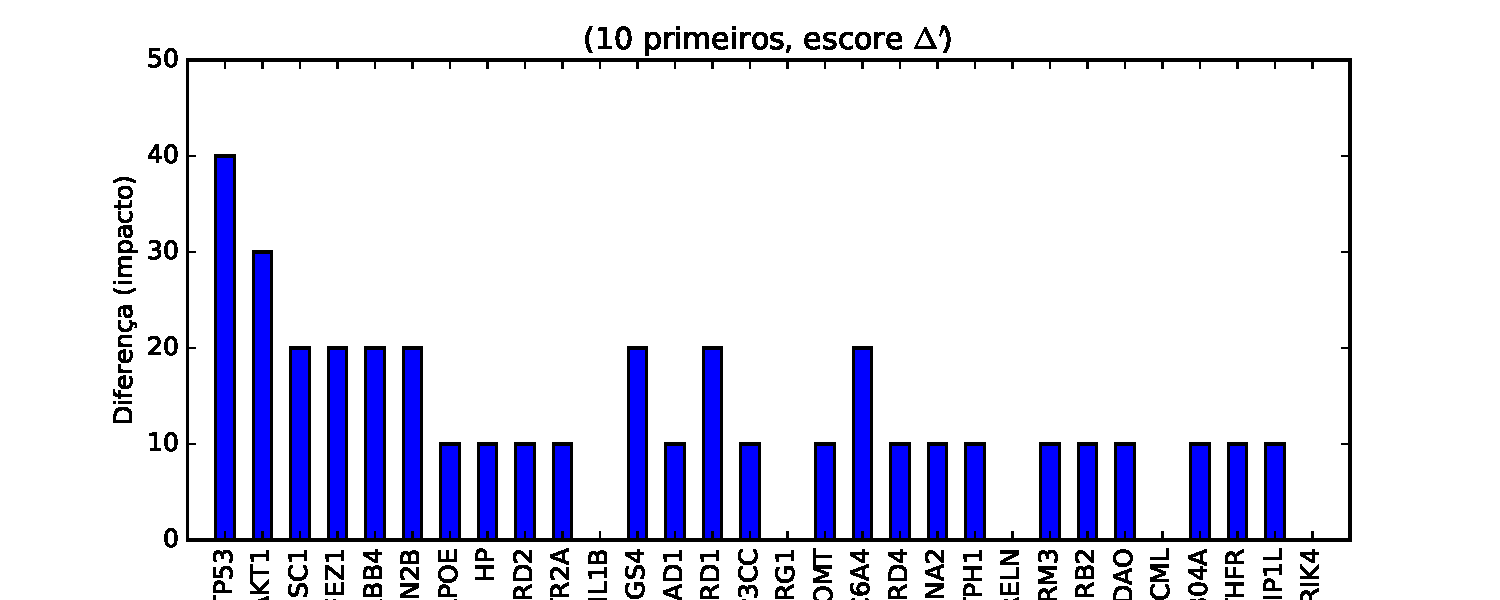
\includegraphics[width=\textwidth]{Images/analyses/fig_LOO_S_10.pdf}
\caption {Análise dos 10 primeiros elementos ordenados por $\Delta'$.
\label{fig_LOO_S_10}}
\flushleft{Fonte: Produzido pelos autores.}
\end{figure}
%

Podemos observar que os genes de maior grau \textbf{\textit{TP53}} (333) e \textbf{\textit{AKT1}} (138), apresentaram impactos um pouco maior que os demais que foram respectivamente de \textbf{\textit{40\%}} e \textbf{\textit{30\%}}.
No entanto, ao comparar com o impacto dos demais genes que não têm graus tão altos, observamos que, de uma forma geral, os impactos não foram diretamente proporcionais aos graus dos genes.
%

Observamos também que os genes \textbf{\textit{IL1B, RELN, NRG1, GRIK4}} e \textbf{\textit{OPCML}} não apresentaram mudanças no resultado em relação ao escore analisada ($\Delta'$), assim como o gene \textbf{\textit{MTHFR}} e os outros que apresentaram \textbf{\textit{10\%}} de diferença dos genes selecionados, comparado ao resultado original do experimento.
Devido a isto, podemos presumir de que tais genes não apresentam uma importância significativa para o método em estudo em relação aos 10 primeiros selecionados utilizando o fator de ranqueamento o escore $\Delta'$.
%

Os genes \textbf{\textit{CHRNA7, DAOA, DTNBP1, MUTED, NPAS3, OFCC1, PRODH}} e \textbf{\textit{SLC18A1}} não foram integrados com a rede PPI.
Ou seja, durante a integração de dados, tais genes não possuíam um nó correspondente na rede PPI e, portanto, não foram utilizados.

Ao analisar os genes mencionados anteriormente \textbf{\textit{TP53}} e \textbf{\textit{AKT1}}, ambos possuem um alto grau na rede gerada pelo método NERI.
E isto pode sugerir que a remoção de um gene com alto grau influencia diretamente no resultado.
%
Por outro lado, os demais genes deram valores bastante parecidos, oscilando entre 0\% à 10\%.
Por exemplo, os genes \textsl{\textbf{ZNF804A}}, \textsl{\textbf{MTHFR}} e \textsl{\textbf{RPGRIP1L}} possuem grau \textsl{\textbf{1}}, e no entanto, causaram \textsl{10\%} de impacto em relação ao experimento original, onde apresenta-se semelhante a remoção do terceiro gene, o \textsl{\textbf{DISC1}} com grau \textsl{91}.
Isso demonstra que a correlação entre o grau e o impacto observado na lista resultante final não é direta. 
%

%
\subsubsection{Análise dos 20 e 50 primeiros elementos}
%
%Imagem
\begin{figure}[ht!]
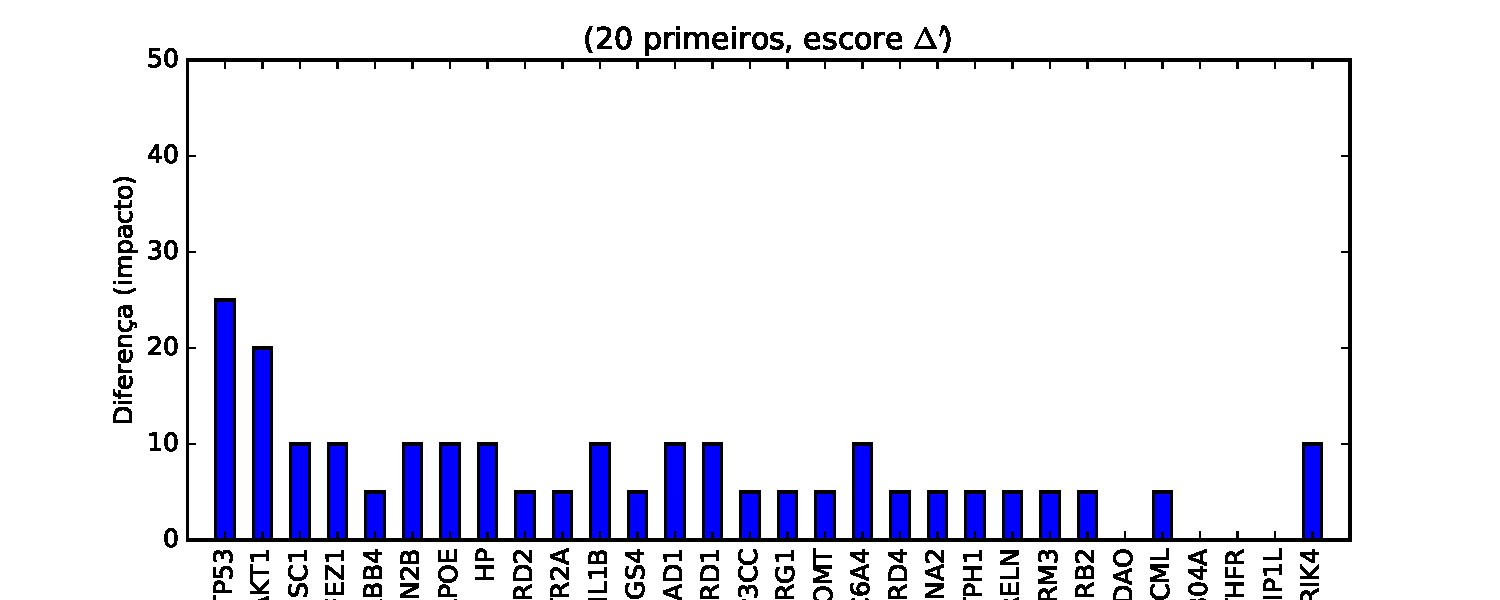
\includegraphics[width=1\textwidth]{Images/analyses/fig_LOO_S_20.pdf}
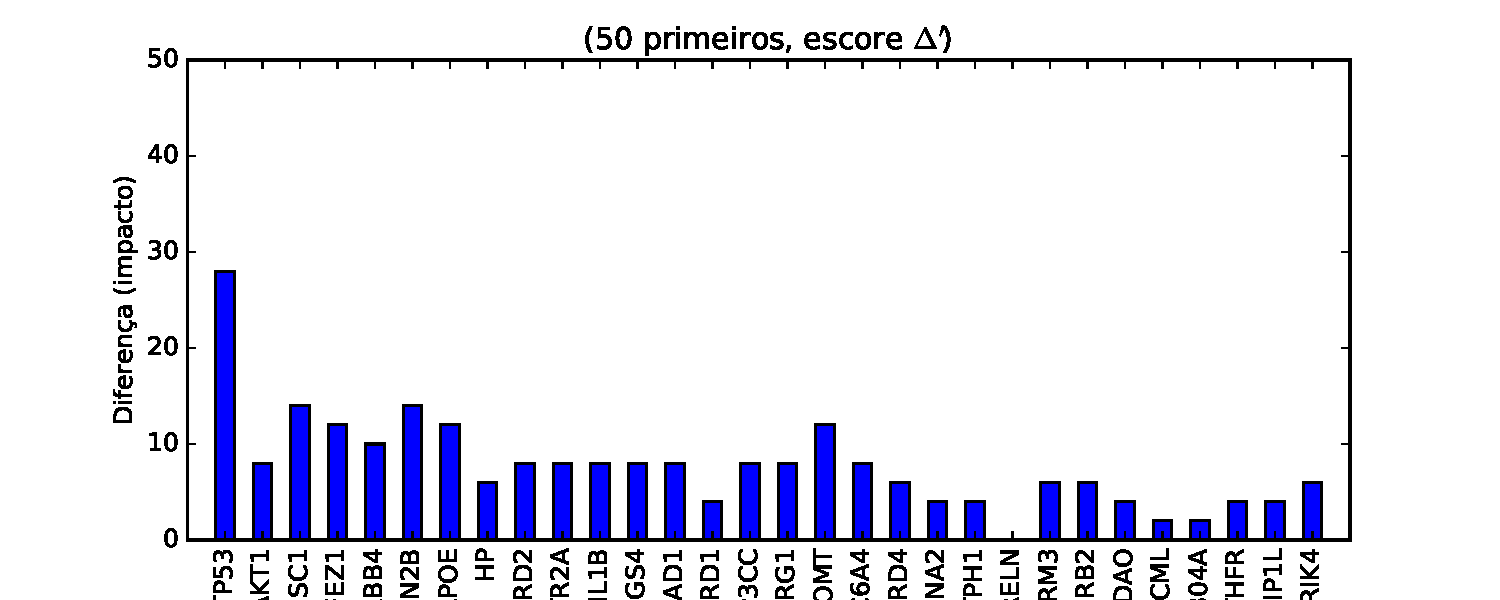
\includegraphics[width=1\textwidth]{Images/analyses/fig_LOO_S_50.pdf}
\caption {Análise dos 20 e 50 primeiros elementos ordenados por $\Delta'$.
\label{fig_LOO_S_20-50}}
\flushleft{Fonte: Produzido pelos autores.}
\end{figure}
%

A figura \ref{fig_LOO_S_20-50} apresenta dois gráficos de forma comparativa, de modo que o de cima representa os \textbf{\textit{20}} primeiros genes ranqueados resultantes em relação ao escore $\Delta'$ e o gráfico de baixo apresenta os \textbf{\texit{50}} primeiros. Sendo eixo \textit{Vertical} a similaridade com o resultado original e o eixo \textit{Horizontal} o gene removido no experimento em questão.
%

A remoção do gene \textbf{\texit{MTHFR}} apresentou baixo impacto: \textbf{\textit{0\%}} de diferença nos primeiros \textbf{\textit{20}} elementos e  \textbf{\textit{5\%}} em relação aos primeiros \textbf{\textit{50}} elementos da lista original.
%
Este mesmo efeito aconteceu na remoção do gene \textbf{\textit{RELN}}, variando de \textbf{\textit{0\%}} de diferença percentual, dos genes selecionados em relação ao experimento original, nos primeiros \textbf{\textit{20}} elementos para \textbf{\textit{5\%}} em relação aos primeiros \textbf{\textit{50}}.
%

Podemos observar também uma diminuição de experimentos com \textbf{\textit{10\%}} ou menos de impacto. Caindo de \textbf{\textit{36}} experimentos ao todo e \textbf{\textit{28}} válidos, para \textbf{\textit{31}} ao todo e \textbf{\textit{23}} válidos (Os experimentos não válidos para análise são os que não integraram com a base de dados \textbf{\textit{GWAS}}, totalizando \textbf{\textit{8}} \textit{genes/experimentos}).
%

O gene \textbf{\textit{TP53}} que causa o maior impacto na similaridade em sua remoção, variou de \textbf{\textit{25\%}} para \textbf{\textit{29\%}} nos respectivos agrupamentos \textbf{\textit{20}} e \textbf{\textit{50}} primeiros genes selecionados. Isso implica que ao analisar \textbf{\textit{30}} elementos a mais, houve um aumento do impacto de \textbf{\textit{4\%}} no pior caso. Sugerindo uma boa robustez do método em relação a remoção de um único gene semente.
%

Outro ponto importante de observação, é o gene \textsl{\textbf{AKT1}} que possui um alto grau na rede gerada pelo método NERI, apresentar uma variação de impacto no resultado bem alta. O impacto apresentado vai de \textsl{\textbf{20\%}} para \textsl{\textbf{8\%}}, nos gráficos representantes dos \textsl{\textbf{20}} e \textsl{\textbf{50}} primeiros genes, respectivamente.
Este fator aponta, mais um vez, que o grau do gene relativo a rede não causa um impacto diretamente proporcional ao grau.

%
\subsubsection{Análise dos 100 e 200 primeiros elementos}
%
%Imagem
\begin{figure}[ht!]
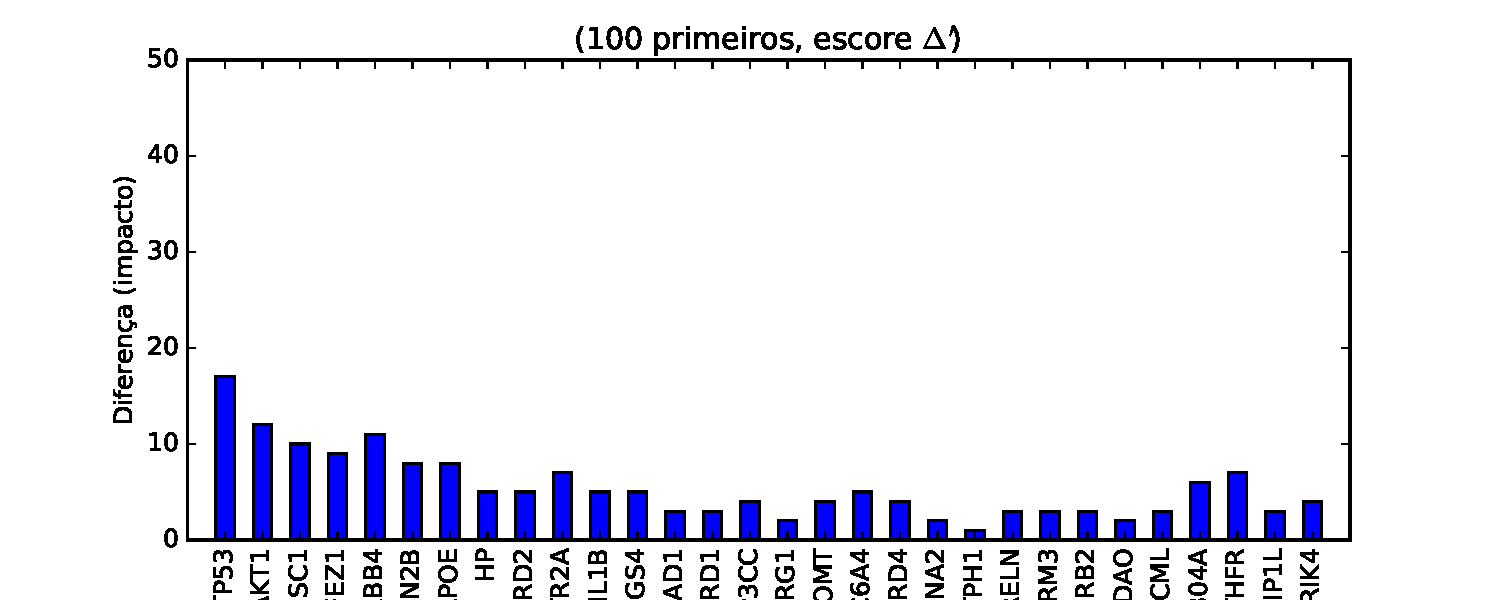
\includegraphics[width=1\textwidth]{Images/analyses/fig_LOO_S_100.pdf}
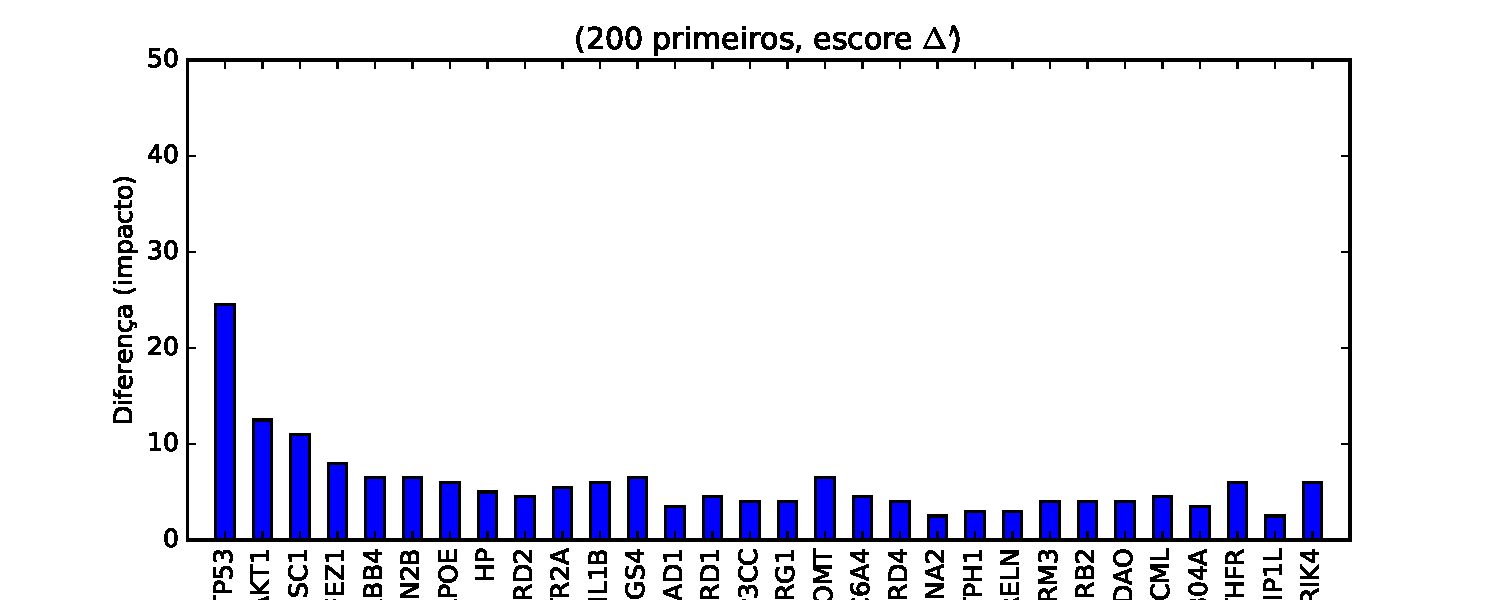
\includegraphics[width=1\textwidth]{Images/analyses/fig_LOO_S_200.pdf}
\caption {Análise dos 100 e 200 primeiros elementos ordenados por $\Delta'$.
\label{fig_LOO_S_100-200}}
\flushleft{Fonte: Produzido pelos autores.}
\end{figure}
%
A imagem \ref{fig_LOO_S_100-200} também apresenta dois gráficos comparativos em relação a similaridade do ranqueamento gênico baseado na quantidade de elementos selecionados. O gráfico de cima, apresenta a diferença em percentual da similaridade dos \textbf{\textit{100}} primeiros genes e o de baixo os primeiros \textbf{\textit{200}}.

%
Podemos observar em ambos os gráficos, que neste ponto de análise não houve remoção de gene que não causou impacto na similaridade dos resultados em relação a amostra original.

%
Um fato importante que ambos os gráficos demonstram, é a mediana dos impactos, onde apresentaram um valor abaixo de \textbf{\textit{10\%}}. Isso demonstra que o impacto gerado pela remoção de um único gene semente varia em torno de \textbf{\textit{10\%}}, o que é muito aceitável em vista da assertividade obtida.

%
Ao observarmos o gene \textbf{\textit{TP53}}, que durante todo o experimento foi o que apresentou maior impacto no resultado, podemos notar que o mesmo apresentou um aumento de \textbf{\textit{17\%}} do impacto para \textbf{\textit{24\%}} ao compararmos os ranqueamentos de \textbf{\textit{100}} e \textbf{\textit{200}} genes. Este valor pode ser considerado baixo, em vista que o numero de elementos da lista analisada foi dobrado e a diferença do impacto gerado foi de \textbf{\textit{7\%}}.

% 
Um comportamento que aparece em ambos os gráficos, que não havia aparecido com tanta nitidez nos anteriores, é a decrescência do impacto da esquerda para direita. Onde os experimentos estão ordenados com relação ao seu grau na rede interna gerada pelo método NERI. Isso implica que mesmo não tendo uma relação direta com o impacto o grau do gene semente apresenta correlação ao analisar uma quantidade maior de genes priorizados do resultado final.

%
%
% ============== X ===============
%
%
\subsection{Estudo dos gráficos em relação ao escore \textit{X}}
%
\subsubsection{Análise dos 10 primeiros elementos}
%
%Imagem
\begin{figure}[ht!]
\centering
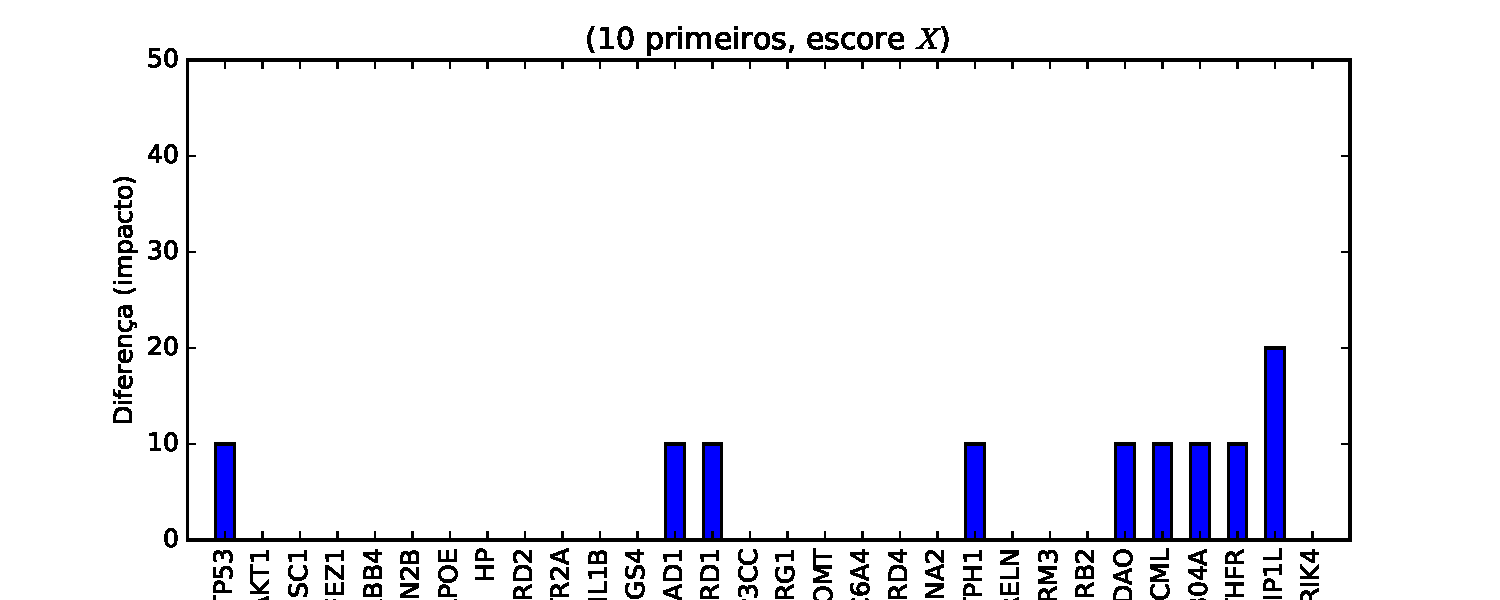
\includegraphics[width=\textwidth]{Images/analyses/fig_LOO_X_10.pdf}
\caption {Análise dos 10 primeiros elementos ordenados por \textit{X}.
\label{fig_LOO_X_10}}
\flushleft{Fonte: Produzido pelos autores.}
\end{figure}
%

%
A figura \ref{fig_LOO_X_10} apresenta um gráfico comparativo referente aos resultados dos experimentos com remoção de apenas \textsl{um gene semente} por vez. O eixo \textbf{Horizontal} representa cada experimento com seu respectivo \textbf{gene semente} removido do agrupamento original, estando estes ordenados  pelo grau que representa na rede gerada pelo método NERI. Sendo esta organização, do maior para o menor no sentido esquerda para direita. O eixo \textsl{Vertical}, por sua vez, representa a \textsl{diferença percentual} dos genes ranqueados em relação ao experimento original, tendo como fator de ordenação o escore \textsl{\textbf{X}}. Por conseguinte, apresentando a comparação dos \textsl{10} primeiros genes ranqueados, sendo estes em relação a remoção do respectivo \textsl{gene semente} apresentado, com os 10 primeiros ranqueados pelo \textsl{experimento original}.
%

Em primeira análise, podemos perceber que o gene semente \textbf{\textsl{RPGRIP1L}} causou o maior impacto em sua remoção, apresentando o percentual de \textsl{\textbf{20\%}} de diferença dos \textsl{\textbf{genes ranqueados}} em relação a amostra original. Este impacto apresenta um comportamento de \textsl{\textbf{outlier}} em relação ao agrupamento de experimentos, em vista que a mediana dos impactos foi de \textsl{\textbf{0\%}}, ou seja, a maior parte dos experimentos em questão não apresentaram diferença entre os \textsl{genes ranqueados} com o \textsl{experimento original}.
%

Podemos observar também que apenas \textsl{\textbf{9}} genes apresentaram impacto em sua remoção. Sendo entre estes, a mediana do impacto \textsl{\textbf{10\%}}, o que é um bom indicador da robustez do método NERI.
%

Um ponto importante para observação é a mudança do gene causador de maior impacto em relação aos \textsl{\textbf{fatores de ranqueamento}}. Quando o ranqueamento foi feito pelo escore \textsl{\textbf{$\Delta'$}} (analisado na seção anterior), o gene semente causador de maior impacto foi \textsl{\textbf{TP53}}, este no qual aprestou apenas \textsl{\textbf{10\%}} de impacto em relação ao escore de ranqueamento \textsl{\textbf{X}}. Isso indica que ambos os genes são impactantes no resultado final do experimento, porém, a abordagem adotada para ranqueamento gênico influencia diretamente na análise.
%


\subsubsection{Análise dos 20 e 50 primeiros elementos}
%
%Imagem
\begin{figure}[ht!]
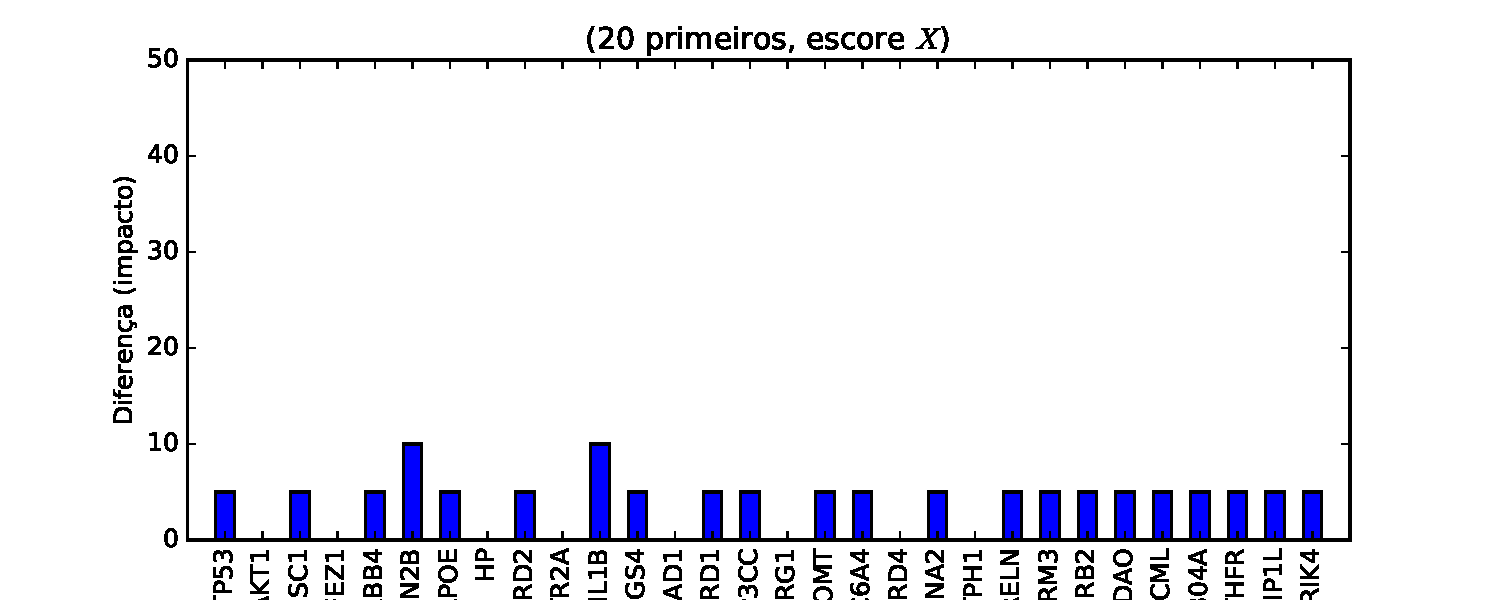
\includegraphics[width=1\textwidth]{Images/analyses/fig_LOO_X_20.pdf}
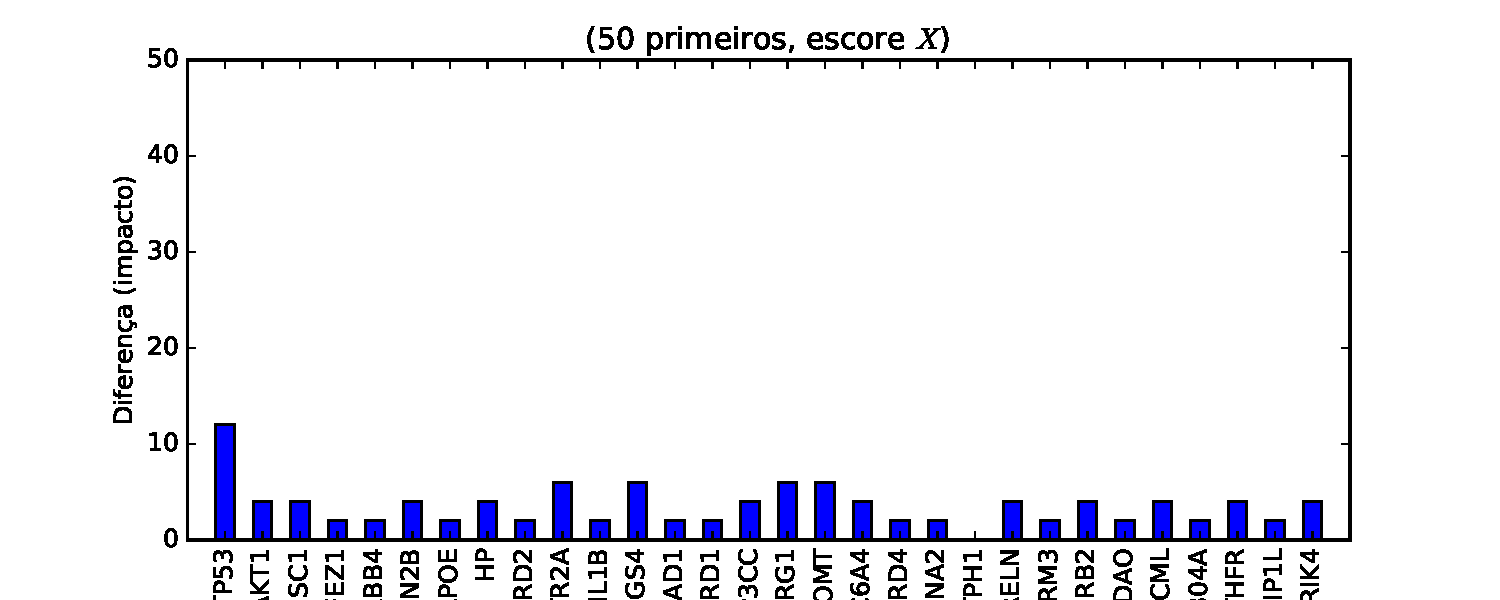
\includegraphics[width=1\textwidth]{Images/analyses/fig_LOO_X_50.pdf}
\caption {Análise dos 20 e 50 primeiros elementos ordenados por \textit{X}.
\label{fig_LOO_X_20-50}}
\flushleft{Fonte: Produzido pelos autores.}
\end{figure}
%

%
A figura \ref{fig_LOO_X_20-50} apresenta dois gráficos comparativos, demonstrando o impacto causado no ranqueamento gênico pelo método NERI ao remover determinados genes sementes. Cada gráfico representa o impacto relativo a quantidade dos genes priorizados analisados, de forma que o eixo \textsl{Horizontal} represente os genes removidos em cada experimento, estando ordenados da esquerda para direita levando em conta grau do gene semente. Assim sendo, o eixo \textsl{Vertical} indica o impacto causado no resultado final em relação a amostra original, este impacto se dá pela diferença percentual de genes presentes no agrupamento experimento e agrupamento original. Estão representados no gráfico de cima, o impacto causado em relação ao ranqueamento dos \textsl{\textbf{20}} primeiros genes, e os \textsl{\textbf{50}} primeiros no gráfico de baixo.

%
Podemos observar em primeira observação, que a quantidade de genes que causaram impacto no ranqueamento gênico. Onde o impacto aumentou consideravelmente logo nos primeiros \textsl{\textbf{20}} genes analisados, sendo \textsl{\textbf{22}} experimentos impactantes. Diferente dos \textsl{\textbf{10}} primeiros, como pode ser visto no gráfico da figura \ref{fig_LOO_X_10}, onde apenas \textsl{\textbf{9}} experimentos apresentaram impacto. Este mesmo comportamento pode ser observado, ao compararmos o gráfico dos \textsl{\textbf{20}} primeiros genes, com o gráfico dos \textsl{\textbf{50}} primeiros. Este ultimo apresenta apenas \textsl{\textbf{1}} experimento que não causou impacto em sua remoção, sendo ele a remoção do gene \textsl{\textbf{TPH1}}.

%
Quando olhamos para o experimento com a remoção do gene \textsl{\textbf{TPH1}}, podemos notar um comportamento atípico. O mesmo apresentou um impacto no ranqueamento gênico de \textsl{\textbf{10\%}} nos primeiros \textsl{\textbf{10}} genes analisados. Porém, nos dois gráficos subsequentes, representando respectivamente \textsl{\textbf{20}} e \textsl{\textbf{50}} primeiros genes ranqueados, o mesmo não apresentou impacto. Ao observarmos este comportamento, podemos inferir que este gene não é de grande importância para o ranqueamento gênico feito pelo método NERI.

%
O gráfico que representa os \textsl{\textbf{20}} primeiros genes ranqueados em relação a \textsl{\textbf{X}}, apresenta uma mediana de impacto de apenas \textsl{\textbf{5\%}}, valor este, considerado muito baixo, em vista que estes são os genes considerados mais importantes pelo método NERI.

%
Uma outra ótica que podemos incutir aos experimentos é a observação em relação ao grau dos genes sementes removidos. Os gráficos demonstram que em relação ao escore \textsl{\textbf{X}}, o grau é um fator altamente impactante no resultado final, em vista que os genes com maior grau \textsl{\textbf{TP53}}, \textsl{\textbf{AKT1}} e \textsl{\textbf{DISC1}} não apresentaram em sua maioria os maires impactos no resultado final. Ficando esta métrica salva apenas para o \textsl{\textbf{TP53}} na análise dos \textsl{\textbf{50}} primeiros genes ranqueados, onde seu impacto é de \textsl{\textbf{22\%}} em relação a amostra original.

%


%
%
\subsubsection{Análise dos 100 e 200 primeiros elementos}
%
%Imagem
\begin{figure}[ht!]
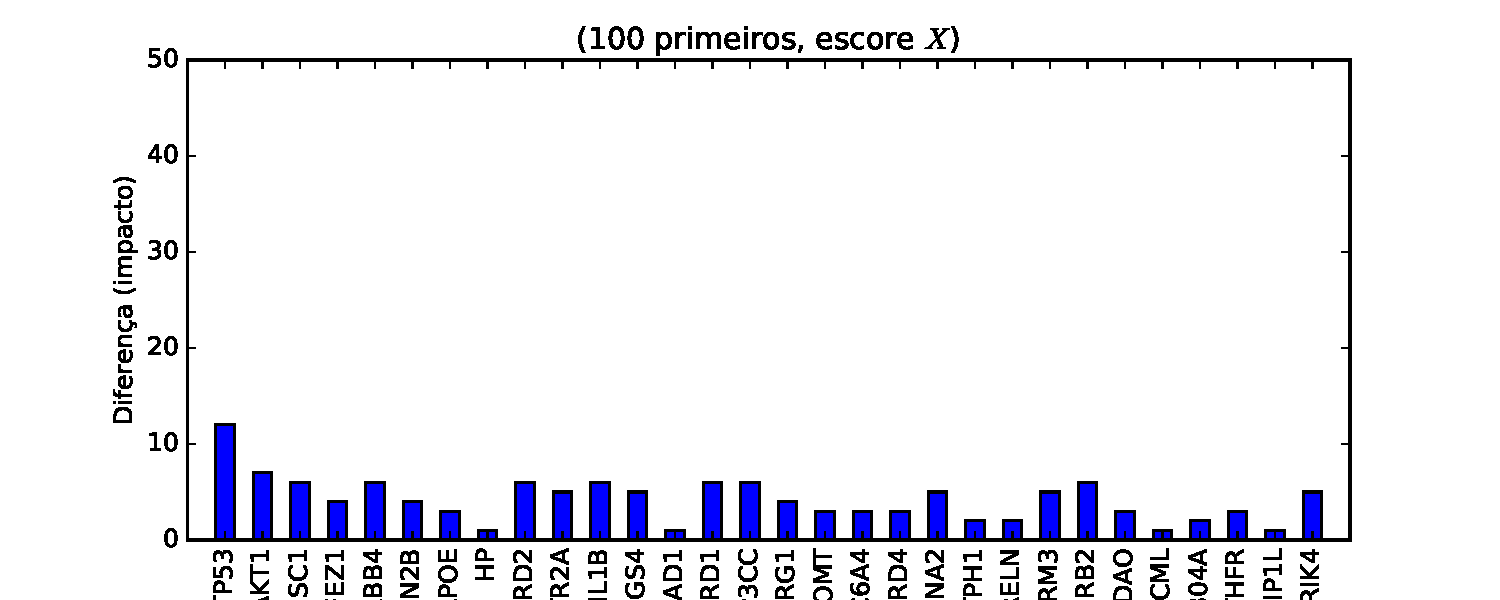
\includegraphics[width=1\textwidth]{Images/analyses/fig_LOO_X_100.pdf}
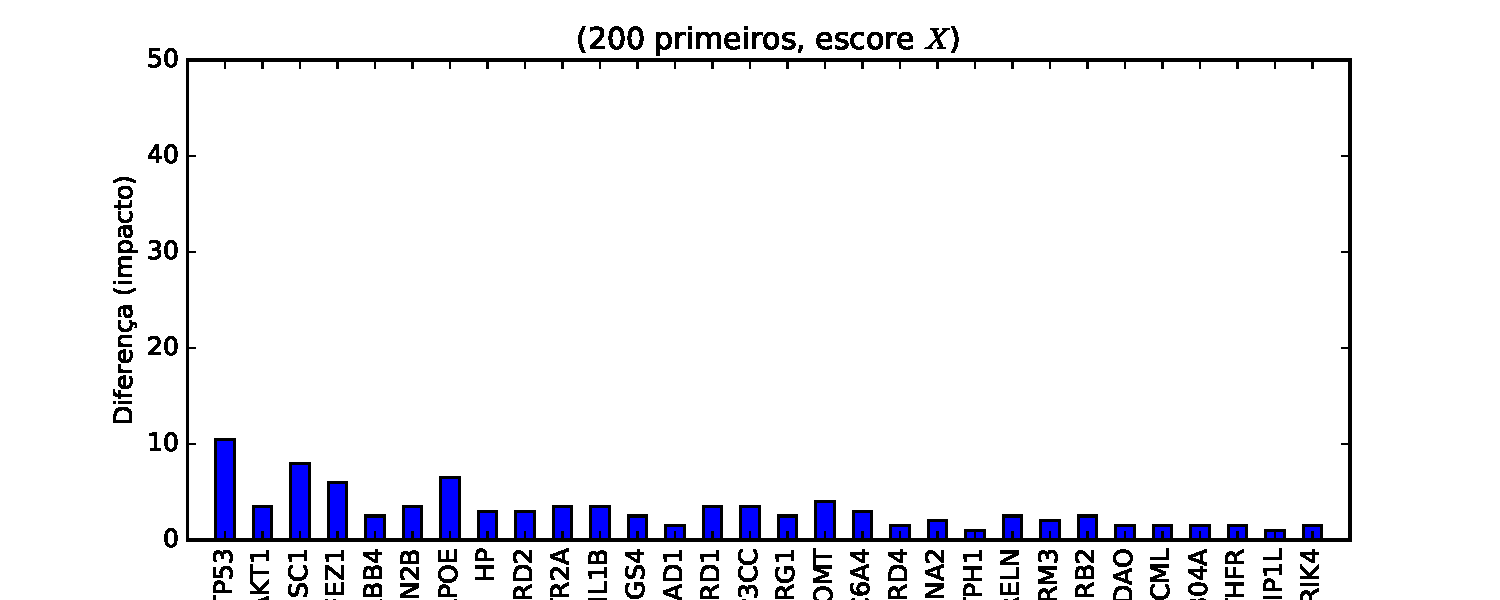
\includegraphics[width=1\textwidth]{Images/analyses/fig_LOO_X_200.pdf}
\caption {Análise dos 100 e 200 primeiros elementos ordenados por \textit{X}.
\label{fig_LOO_X_100-200}}
\flushleft{Fonte: Produzido pelos autores.}
\end{figure}
%
%

A Figura~\ref{fig_LOO_S_100-200} apresenta dois gráficos comparativos em relação ao impacto representado pela remoção do \textsl{\textbf{gene semente respectivo}}. Estes gráficos podem ser lidos da mesma forma que os apresentados anteriormente nesta sessão, onde o de cima representa os primeiros \textsl{\textbf{100}} genes ranqueados e o de baixo os \textsl{\textbf{200}} primeiros.
%

Um comportamento que podemos observar ao analisar os dois gráficos apresentados, é a diminuição do impacto geral causado pela remoção dos genes sementes encontrados nos primeiros \textsl{\textbf{200}} genes ranqueados. Esta diminuição no impacto se dá pelo aumento da lista de genes ranqueados, de forma que mais genes em comum estejam nas listas geradas pelos experimentos e na lista do experimento original. Este comportamento indica uma tendência de diminuição do impacto em relação ao tamanho da lista analisada, porém, o gene semente causador de maior impacto em sua remoção ainda se mantém, sendo \textsl{\textbf{TP53}} com \textsl{\textbf{12\%}} e \textsl{\textbf{10\%}} de impacto nos gráficos de \textsl{\textbf{100}} e \textsl{\textbf{200}} genes ranqueados respectivamente.

Também podemos notar um limiar de impacto abaixo de \textsl{\textbf{10\%}}, ou seja, a maioria dos experimentos causaram um impacto igual ou inferior a \textsl{\textbf{10\%}} no resultado final em relação a remoção do gene semente respectivo. Este comportamento é um bom indicativo para a robustez do método, em vista que o mesmo se mostra com baixa variação no resultado em relação a remoção de um único gene semente, quando o fator de ranqueamento é o escore $X$.

%
%
% ============== OBS ===============
%
%
\subsection{Observações}
%
Em relação ao método de validação de \textit{remoção de um único gene}, o método NERI apresentou bons resultados de robustez. De forma que o maior impacto encontrado pela remoção de um único gene semente foi de \textit{\textbf{40\%}} em relação ao escore $\Delta'$. Porém  a mediana das correlações com o mesmo escore de ranqueamento, foi de \textit{\textbf{20\%}} em relação aos \textbf{\textit{10}} primeiros elementos. Estes valores melhoram ao observar o ranqueamento em relação ao escore $X$, apresentando o maior valor de impacto em \textsl{\textbf{20\%}} com o gene \textsl{\textbf{GRIP1L}}. Fato este que chama atenção por ser um gene semente diferente do maior causador de impacto em relação ao escore $\Delta'$, o gene semente \textsl{\textbf{TP53}}. A mediana de impacto nos primeiros \textsl{\textbf{10}} genes ranqueados pelo escore $X$ foi de \textsl{\textbf{0\%}}, ou seja, a remoção de mais da metade dos genes sementes individualmente não causou impacto no resultado final. Isso significa que os na maioria dos casos os genes ranqueados tanto nos experimentos quanto na amostra original foram os mesmos.

%
% Falar sobre a metrica X também
%

Também deve-se levar em conta que o maior impacto encontrado relação aos \textbf{\textit{200}} primeiros genes selecionados pelo escore $\Delta'$, foi de \textbf{\textit{24\%}} apresentando melhora em relação a análise dos \textbf{\texit{10}} primeiros. A medina apresentou uma queda significativa de \textbf{\texit{20\%}} para \textbf{\textit{5\%}}, o que indica uma convergência de genes selecionados da amostra original com os experimentos. Esse tipo de convergência é esperado com o aumento da quantidade de elementos ranqueados, pois a probabilidade de um gene ser selecionado aumenta proporcionalmente ao tamanho do agrupamento de seleção final. Porém, esta premissa não invalida a eficiência do método em questão, em vista que a quantidade de genes possíveis a serem selecionados é muito maior que a lista dos genes ranqueados.
%
Assim sendo, podemos concluir que o método é robusto em relação a retirada de um único gene semente. Porém, para determinar melhor a robustez do método em análise, há a necessidade de estudar os resultados dos outros modelos de validação empregadas neste trabalho.
%
%
% ======================== CROSS VALIDATION ========================
%
%
\section{Remoção de vários genes sementes}
%
Nesta etapa analisaremos os resultados do método de \textit{Remoção de vários gene sementes}, onde como principal meio de apresentação de dados será o estudo dos gráficos gerados e a discussão de suas interpretações.

\subsection{Esperado}
%
O esperado na utilização do método da \textit{Remoção de mais de um gene} é a capacidade de mapear o impacto causado no resultado final baseado na identificação da quantidade de genes sementes removidos em relação a amostra original. Desta forma observar o impacto causado, a medida que conjuntos de tamanhos diferentes são testados. Com este estudo, podemos aproximar um limiar de confiança no método NERI. Para podermos ter uma análise mais precisa dos resultados, cruzaremos os dados encontrados com os dados gerados pela \textit{Remoção de um único gene}, de forma que consigamos entender melhor o comportamento dos resultados apresentados.
%
%
% ===== S =====
%
%
\subsection{Estudo dos gráficos em relação ao escore $\Delta'$}
%
\subsubsection{Análise dos 10 primeiros elementos}
%
%Imagem
\begin{figure}[ht!]
\centering
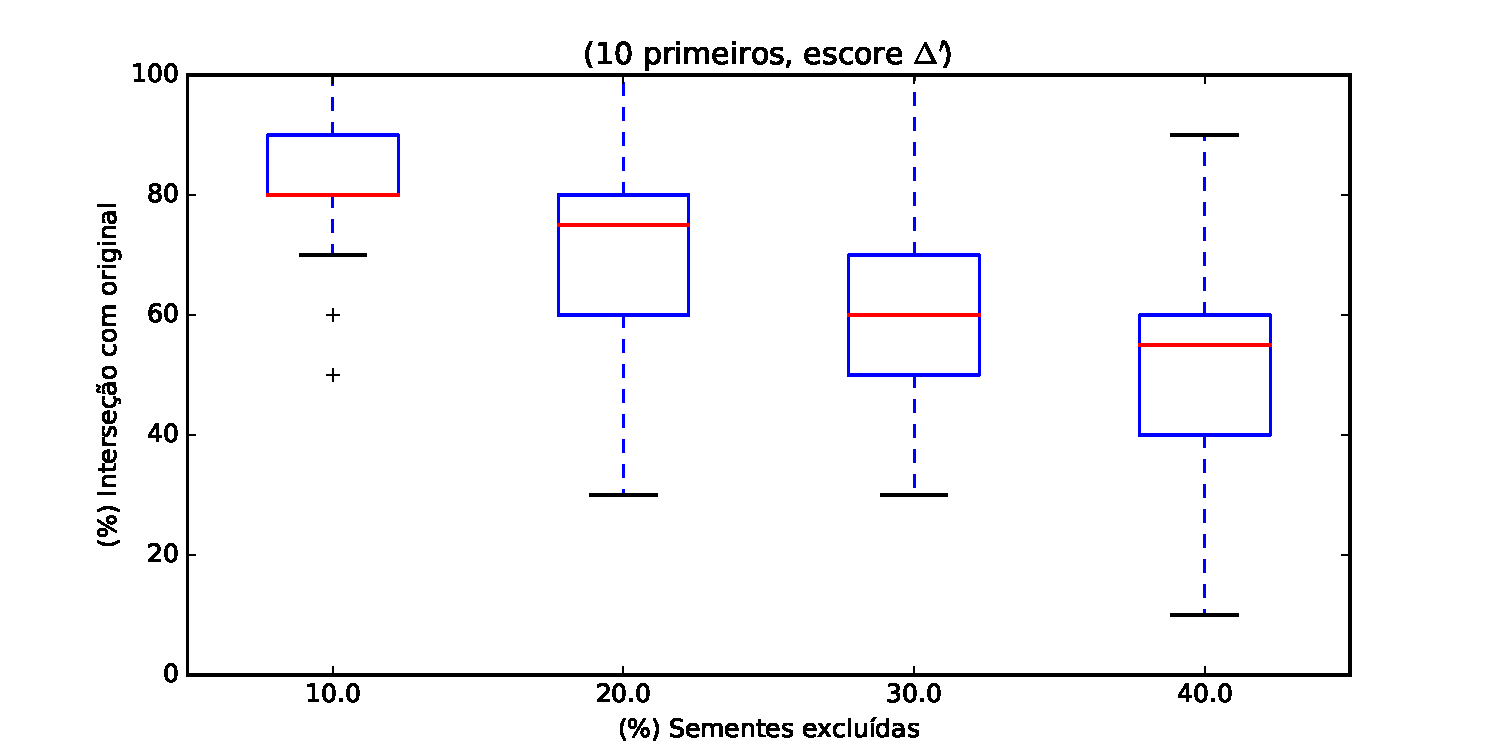
\includegraphics[width=\textwidth]{Images/analyses/fig_S_10_40.pdf}
\caption {Análise dos 10 primeiros elementos ordenados por $\Delta'$.
\label{fig_S_10_40}}
\flushleft{Fonte: Produzido pelos autores.}
\end{figure}
%

%
A Figura~\ref{fig_S_10_40} apresenta um gráfico comparativo dos experimentos utilizando o método \textit{Remoção de mais de um gene}, onde o eixo \textsl{Horizontal} representa a porcentagem de sementes excluídas em relação a amostra original, e o eixo \textsl{Vertical}, por sua vez, representa a porcentagem da interseção dos resultados dos \textsl{\textbf{10}} primeiros genes em relação aos \textsl{\textbf{10}} primeiros apresentados na amostra original, tendo como fator de ranqueamento ao escore $\Delta'$.
%

Conforme podemos observar, a medida que aumentamos o percentual de sementes excluídas, ocorre uma redução gradual na mediana do percentual de interseção de genes selecionados.
Conforme esperado, isso demonstra que a quantidade de genes sementes excluídas influencia diretamente no resultado do experimento.
%

%
Podemos observar também que, a mediana do experimento com a maior porcentagem de remoção apresenta o valor aproximado \textsl{\textbf{50\%}} de interseção, esta métrica é um bom indicativo da robustez do método ao informar que mesmo removendo \textsl{\textbf{40\%}} dos genes sementes, os genes ranqueados pelo método ainda se mantém acima de \textsl{\textbf{50\%}} iguais aos ranqueados pelo método com todos os genes sementes.

Por este gráfico representar somente os \textsl{\textbf{10}} primeiros genes selecionados, esperava-se um impacto no resultado final consideravelmente alto devido ao fato do mesmo apresentar poucos genes em relação ao tamanho da rede \textsl{\textbf{9.554}} Genes (nós). Porém, ao contrário do que imaginávamos, os genes selecionados foram muito próximos da amostra original. Porém a sua precisão varia consideravelmente de modo que a podemos observar que as diferenças entre os limites superiores e inferiores dos experimentos são altas. Isto se dá devido ao tamanho da lista de genes priorizados analisada.
%

Um ponto que chama bastante atenção ao analisar este gráfico, é o boxplot que representa \textbf{\textsl{40\%}} dos genes sementes removidos. O mesmo, apresenta uma variação entre o lime inferior e o limite superior de \textbf{\textsl{60\%}}, ou seja, a bateria de experimentos representados pelo gráfico possui experimentos de similaridade variada entre \textbf{\textsl{20\%}} a \textbf{\textsl{80\%}}. Fato este implica em uma não confiança nos dados representados por este, o comportamento apresentado é reforçado ao fazer uma análise dos \textbf{\textsl{outliers}}. Encontrando um experimento com \textbf{\textsl{90\%}} de similaridade e em contrapartida, um experimento com apenas \textbf{\textsl{10\%}} sendo o menor de todo o estudo em relação aos \textbf{\textsl{10}} primeiros genes removidos.

\subsubsection{Análise dos 20 e 50 primeiros elementos}
%Imagem
\begin{figure}[ht!]
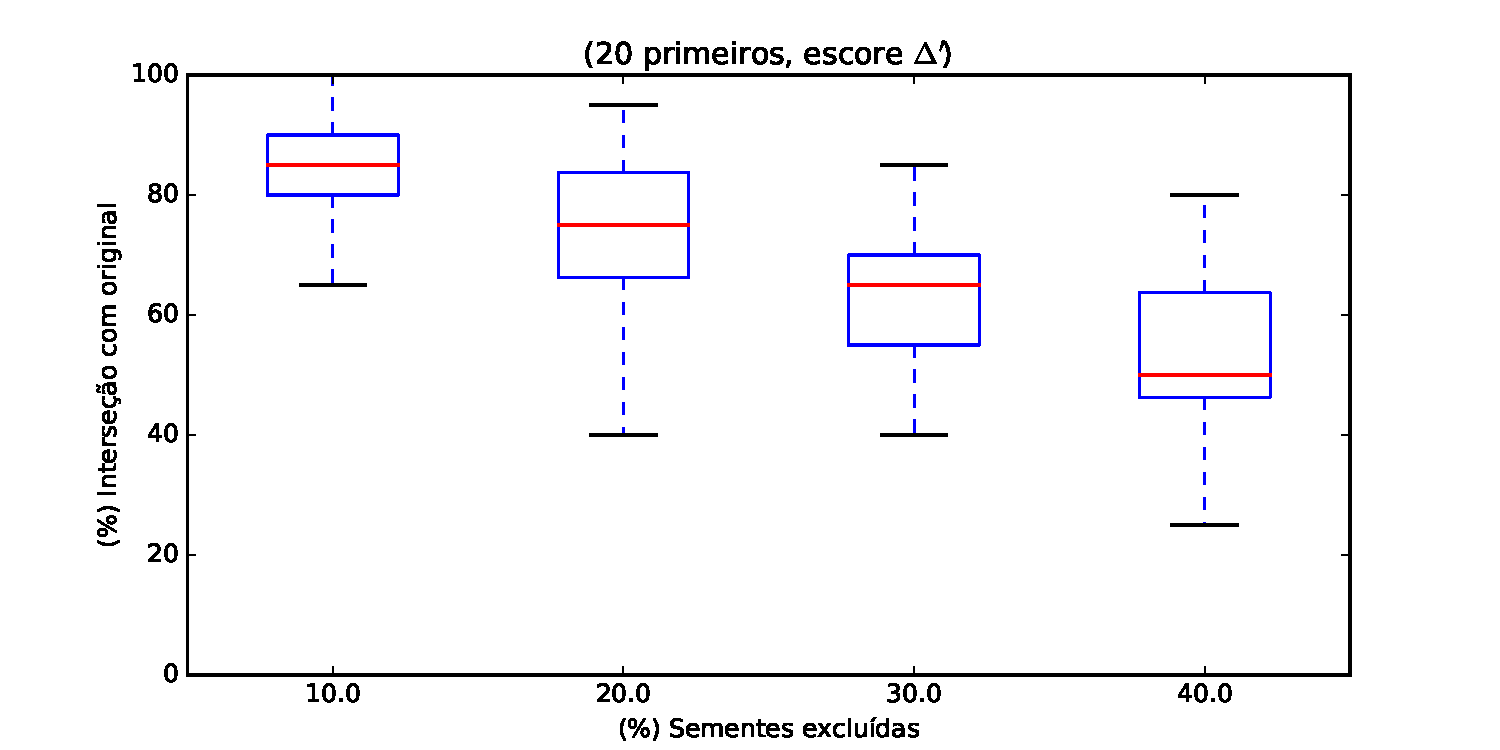
\includegraphics[width=1\textwidth]{Images/analyses/fig_S_20_40.pdf}
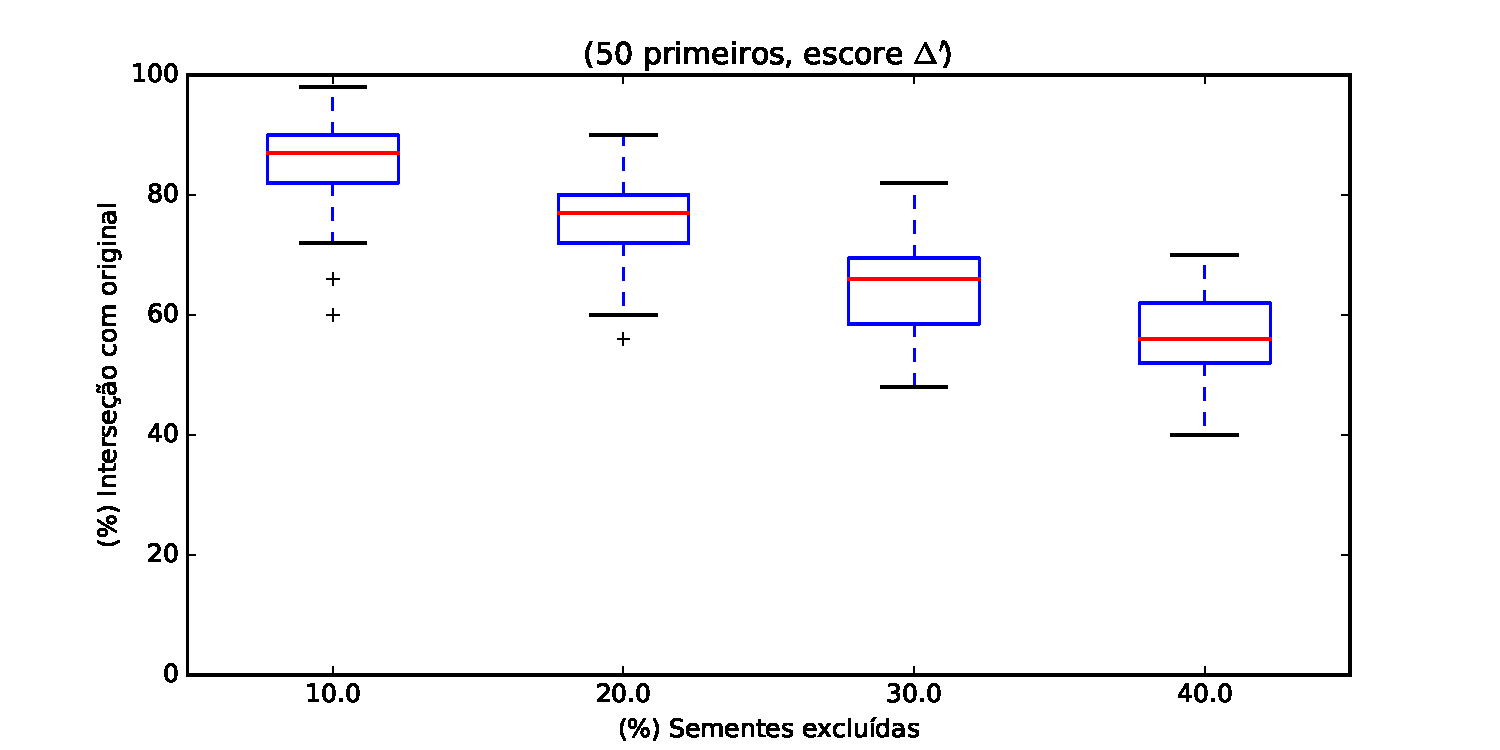
\includegraphics[width=1\textwidth]{Images/analyses/fig_S_50_40.pdf}
\caption {Análise dos 20 e 50 primeiros elementos ordenados por $\Delta'$.
\label{fig_S_20-50_40}}
\flushleft{Fonte: Produzido pelos autores.}
\end{figure}
%

A Figura~\ref{fig_S_20-50_40} apresenta dois gráficos comparativos, sendo o de cima representando a correlação com os \textsl{\textbf{20}} primeiros genes selecionados e de baixo com os primeiros \texit{\textbf{50}}. 
%

Podemos observar no primeiro gráfico a baixa variação da mediana, porém houve uma diminuição na \textit{amplitude interquartílica}. Isto demonstra uma possível convergência de resultados em relação aos dois gráficos. Este fator pode ser observado no \textit{boxplot} referente a \textbf{\textsl{20\%}} do gráfico de cima, onde este representa \textsl{\textbf{20}} primeiros genes selecionados. Neste caso, \textit{amplitude interquartílica} varia de \textit{68\%} a \textit{82\%}, totalizando \textit{14\%} de faixa de variação. No gráfico de baixo, representando os \textbf{\textit{50}} primeiros genes selecionados. Neste caso, há uma variação na \textsl{amplitude interquartílica} de \textbf{\textsl{73\%}} a \textbf{\textsl{80\%}}, totalizando uma faixa de variação de \textbf{\textsl{7\%}}, valor este que apresenta-se metade do valor do gráfico anterior. Esta queda de amplitude remete ao comportamento de convergência, assim representando uma segurança nos resultados apresentados, partindo do princípio de que quanto menor a variação dos resultados, maior é a precisão da medição.
%

Podemos observar também alguns experimentos que ficaram fora do agrupamento, este comportamento é definido como \textit{outlier}. Para entender o porque destes experimentos terem sido apresentados unanimamente com menores resultados do que o corpo amostral, cruzamos os seus dados com os obtidos pela etapa de \textit{remoção de um único gene}. Com este cruzamento de dados, observamos se os genes removidos nestes experimentos contém um ou mais genes que possuem os maiores \textsl{\textsl{graus de impacto}} no resultado.
%

% VERIFICAR QUAIS FORAM OS CASOS DENTRO DO CODIGO
Em 10 experimentos essa premissa apresentou-se verdadeira, resultando menores correlações, onde nestes casos observou-se a falta dos genes sementes \textbf{\textsl{TP53}} e \textbf{\textsl{AKT1}}. Onde ambos causaram o maior impacto no resultado final ao serem removidos sozinhos do experimento (como foi mencionado na sessão anterior). Estes casos apontam uma correlação do impacto acumulativo da remoção de genes sementes no resultado final.
%%%%%
%
%
%
\subsubsection{Análise dos 100 e 200 primeiros elementos}
%
%Imagem
\begin{figure}[ht!]
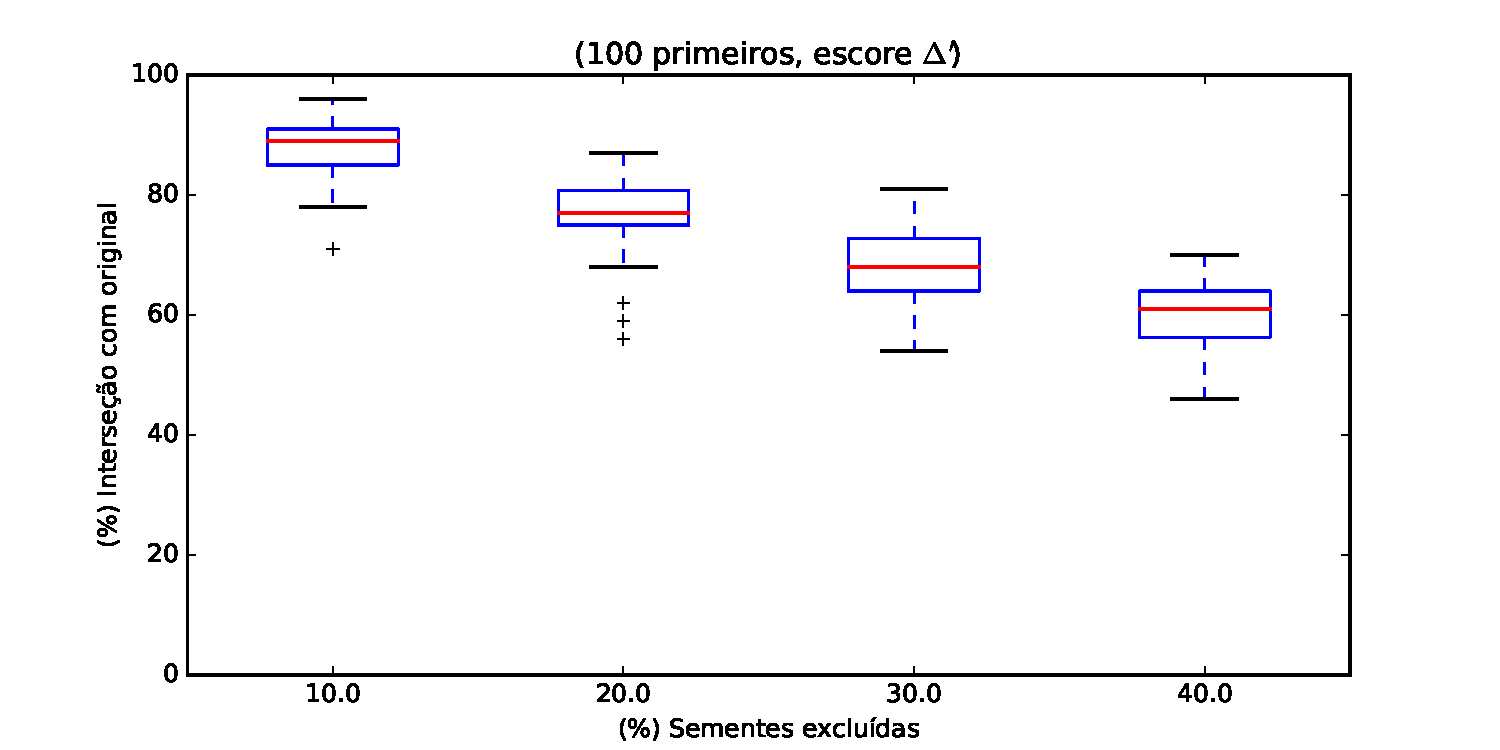
\includegraphics[width=1\textwidth]{Images/analyses/fig_S_100_40.pdf}
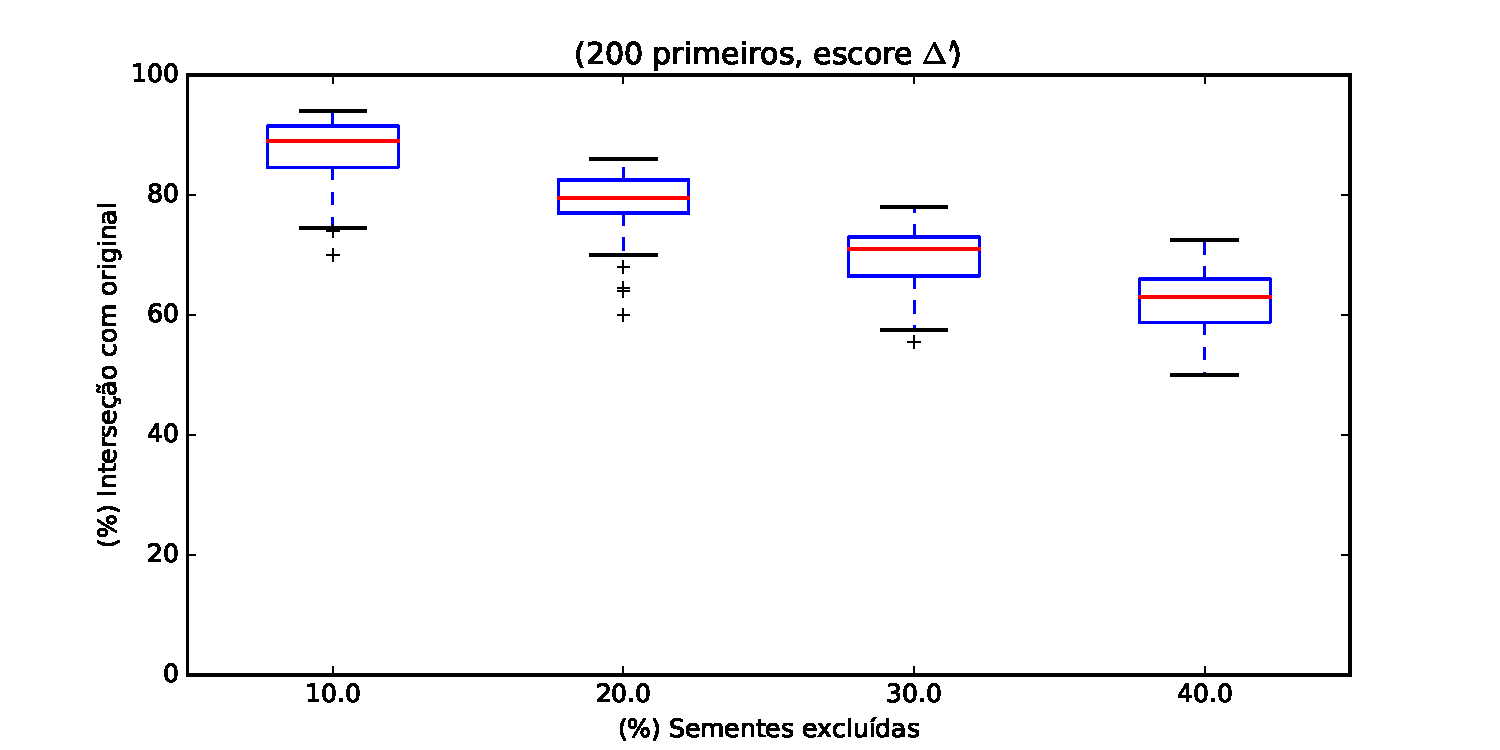
\includegraphics[width=1\textwidth]{Images/analyses/fig_S_200_40.pdf}
\caption {Análise dos 100 e 200 primeiros elementos ordenados por $\Delta'$.
\label{fig_S_100-200_40}}
\flushleft{Fonte: Produzido pelos autores.}
\end{figure}
%%
%

A figura \ref{fig_S_100-200_40} apresenta dois gráficos comparativos entre agrupamentos de experimentos com variação na quantidade de genes sementes. O gráfico \textsl{de cima}, representa a comparação dos \textsl{\textbf{100}} primeiros genes ranqueados em relação ao escore $\Delta'$, onde o eixo \textsl{Horizontal} define os \textsl{boxplots} correspondentes as suas determinadas porcentagens de retirada dos \textsl{\textbf{genes sementes}}. Assim sendo, o eixo \textsl{Vertical} define a porcentagem de interseção dos genes ranqueados pelos experimentos em relação ao experimento original.
Seguindo esta mesma organização, o gráfico \textsl{de baixo} representa os \textsl{\textbf{200}} primeiros genes ranqueados.
%

Podemos notar claramente, que o decrescimento correlacional está presente nos dois gráficos. Ou seja, a correlação dos \textsl{\textbf{genes ranqueados}} cai em mesma proporção nos dois gráficos conforme a quantidade de \textsl{\textbf{genes sementes}} são reduzidas. Porém, podemos enxergar que a \textsl{\textbf{amplitude interquartílica}} respectiva entre os gráficos apresenta uma diminuição. Este aspecto representa bons resultados, pois indica que há uma convergência de resultados conforme o aumento dos \textsl{\textbf{genes ranqueados}} observados.
%

Nesta comparação, podemos observar novamente comportamentos de \textsl{\textbf{outlier}} presentes nos gráficos. Como na análise anterior, os agrupamentos que apresentaram menor correlação, foram os que não tinham em seu agrupamento de \textsl{\textbf{genes sementes}} os mais impactantes observados na etapa de \textsl{\textbf{retirada de uma único gene semente}}, sendo eles \textsl{\textbf{TP53}} e \textsl{\textbf{AKT1}}.
%

Um forte fator de análise é a comparação entre o gráfico dos \textsl{\textbf{10}} primeiros genes ranqueados (\ref{fig_S_10_40}) com o gráfico dos \textsl{\textbf{100}} (\ref{fig_S_100-200_40}). Podemos observar que a mediana subiu de \textsl{\textbf{80\%}} de correlação com a amostra original, para \textsl{\textbf{90\%}} ao comparar os \textsl{\textbf{boxplots}} pertencentes a \textsl{\textbf{10\%}} de remoção. Este fato aponta para uma robustez do método analisado, em vista que fortalece ainda mais o efeito de convergência observado anteriormente. Ao comparar com o gráfico dos \textsl{\textbf{200}} genes ranqueados, notamos que a \textsl{\textbf{mediana}} se mantém a mesma em relação a dos \textsl{\textbf{100}}, indicando que esta convergência ocorre entre nos primeiros \textsl{\textbf{100}} genes ranqueados, sendo este um número muito bom. O mesmo pode ser observado ao comparar os outros \textsl{\textbf{boxplots}} respectivos, os valores apresentados não são os mesmos, mas apresentam um padrão muito próximo de variação.



%
%%%%%
%
%
% ===== X =====
%
%
\subsection{Estudo dos gráficos em relação ao escore \textit{X}}
\subsubsection{Análise dos 10 primeiros elementos}
%
%Imagem
\begin{figure}[ht!]
\centering
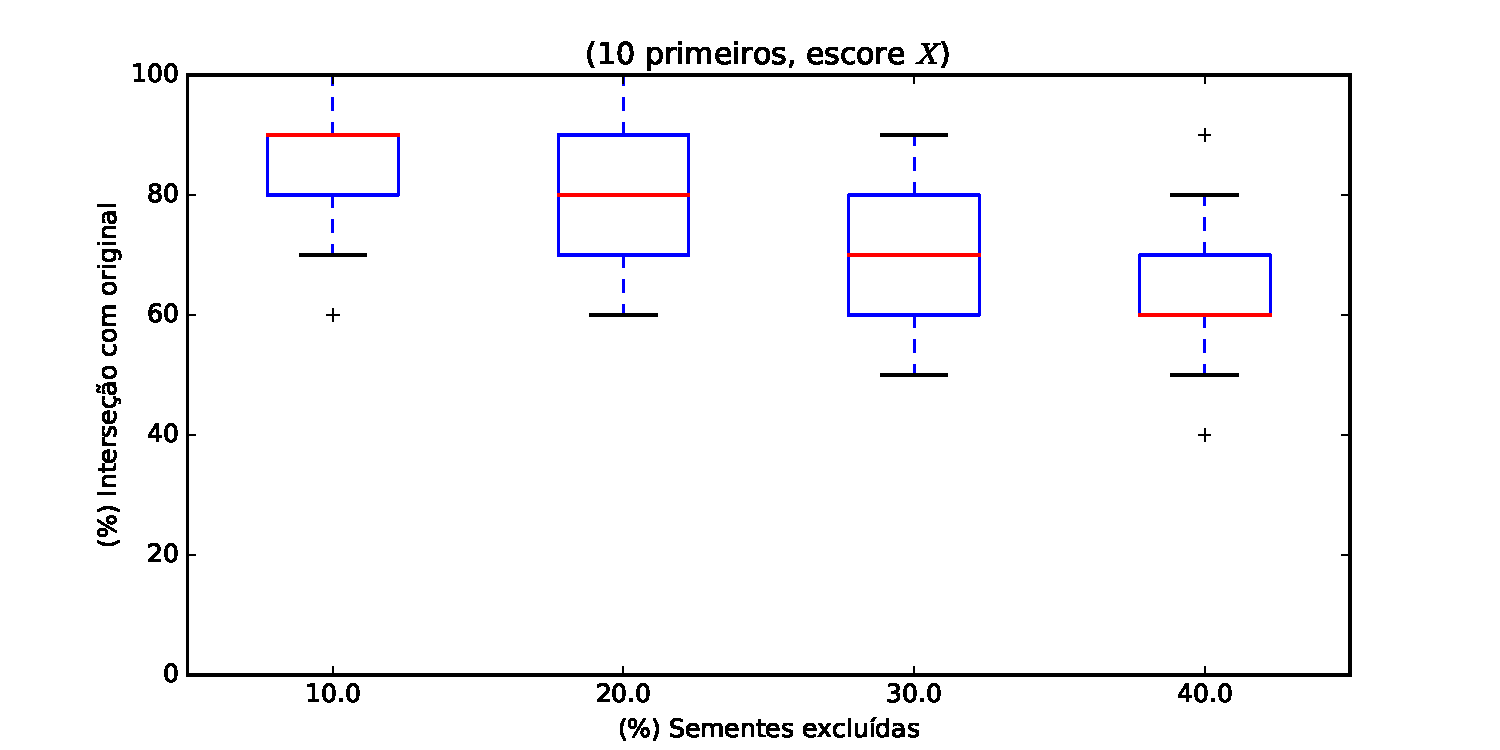
\includegraphics[width=\textwidth]{Images/analyses/fig_X_10_40.pdf}
\caption {Análise dos 10 primeiros elementos ordenados por \textit{X}.
\label{fig_X_10_40}}
\flushleft{Fonte: Produzido pelos autores.}
\end{figure}
%
%

%
A Figura~\ref{fig_X_10_40} apresenta um gráfico comparativo dos experimentos utilizando o método \textit{Remoção de mais de um gene}, onde o eixo \textsl{Horizontal} representa a porcentagem de sementes excluídas em relação a amostra original, e o eixo \textsl{Vertical}, por sua vez, representa a porcentagem da interseção dos resultados dos \textsl{\textbf{10}} primeiros genes em relação aos \textsl{\textbf{10}} primeiros apresentados na amostra original, tendo como fator de ranqueamento o escore $X$.
%
Em primeira análise, fica claro que, assim como o ranqueamento pelo escore de ranqueamento $\Delta'$, quanto maior a quantidade de genes sementes removidos nos experimentos, a correlação das listas de priorização gênica diminui. Fator este esperado, em vista que o método NERI utiliza os genes sementes para realizar a priorização gênica.
%

Ao compararmos este gráfico com o apresentado na análise do escore $\Delta'$ como pode ser vista na Figura~\ref{fig_S_10_40}, podemos notar que a variação dos resultados dos experimentos é muito menor, indicando que o escore $X$ tende a ser mais robusto. O boxplot que intuitivamente apresentaria maior diferença de limite superior e inferior, o referente a \textbf{\textsl{40\%}} de remoção de genes sementes, não apresentou uma grande variação. Este comportamento é o contrário do observado anteriormente, onde a variação anterior apresentou-se em \textbf{\textsl{60\%}}, diferentemente do gráfico em relação ao escore \textbf{$X$} apresentando \textbf{\textsl{30\%}}, metade do valor anterior. Sugerindo mais uma vez a robustez do escore de ranqueamento $X$ superior ao escore $\Delta'$.

Podemos notar que a mediana do pior caso ficou em \textbf{\textsl{60\%}} de similaridade com a lista de genes ranqueados em relação ao experimento original. O pior caso sendo determinado intuitivamente pelo conjunto de experimentos com  \textbf{\textsl{40\%}} de remoção dos genes sementes em relação ao experimento original. A variação entre a menor e maior mediana, sendo elas respectivamente \textbf{\textsl{60\%}} e \textbf{\textsl{90\%}}, apresenta-se em \textbf{\textsl{30\%}}. Um valor muito bom se levarmos em consideração que no pior caso foram removidos \textbf{\textsl{40\%}} dos genes sementes da amostra original, ou seja, a variação do impacto proporcional causado foi menor que o fator de remoção de genes sementes em relação a amostra original. Isto indica uma boa robustez do método NERI em relação ao fator de ranqueamento $X$.  

\subsubsection{Análise dos 20 e 50 primeiros elementos}
%
%Imagem
\begin{figure}[ht!]
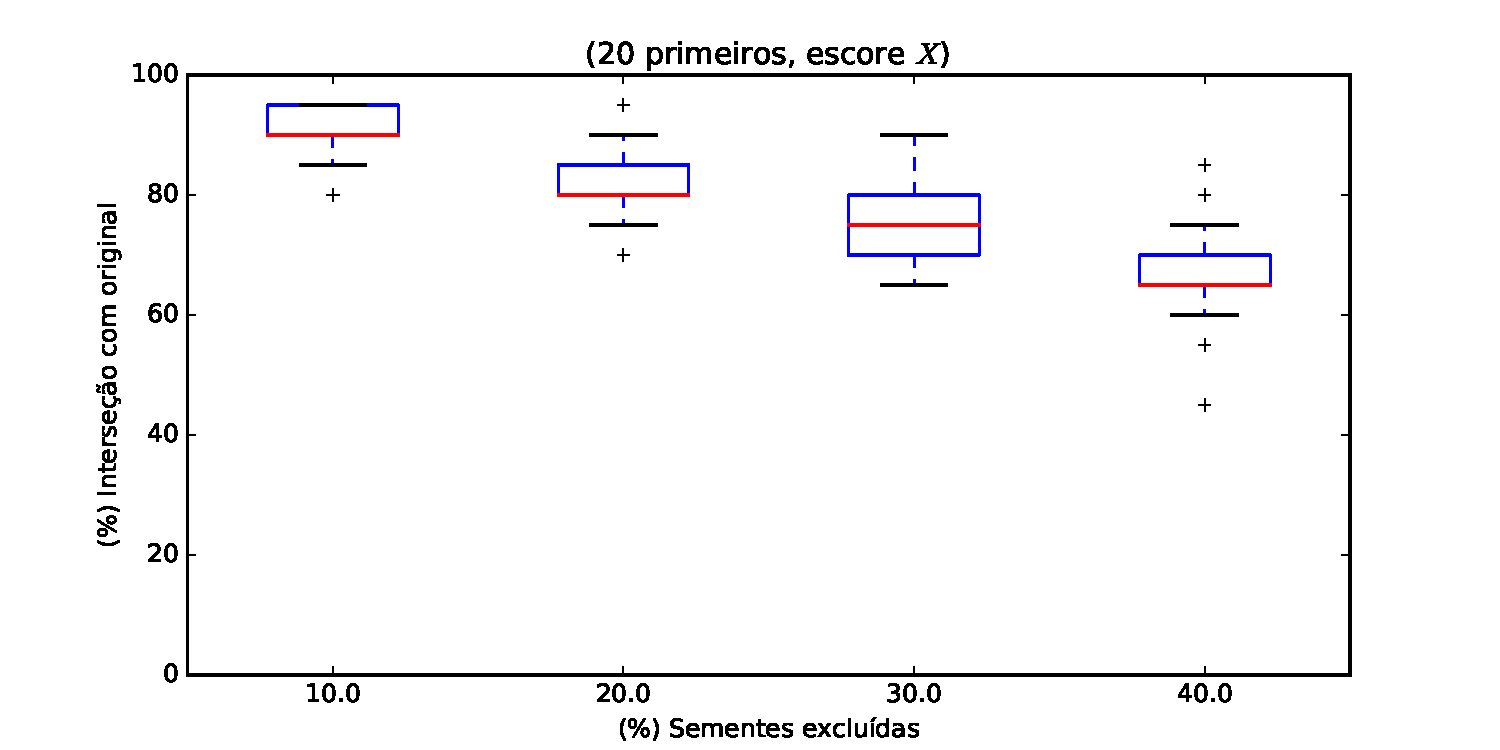
\includegraphics[width=1\textwidth]{Images/analyses/fig_X_20_40.pdf}
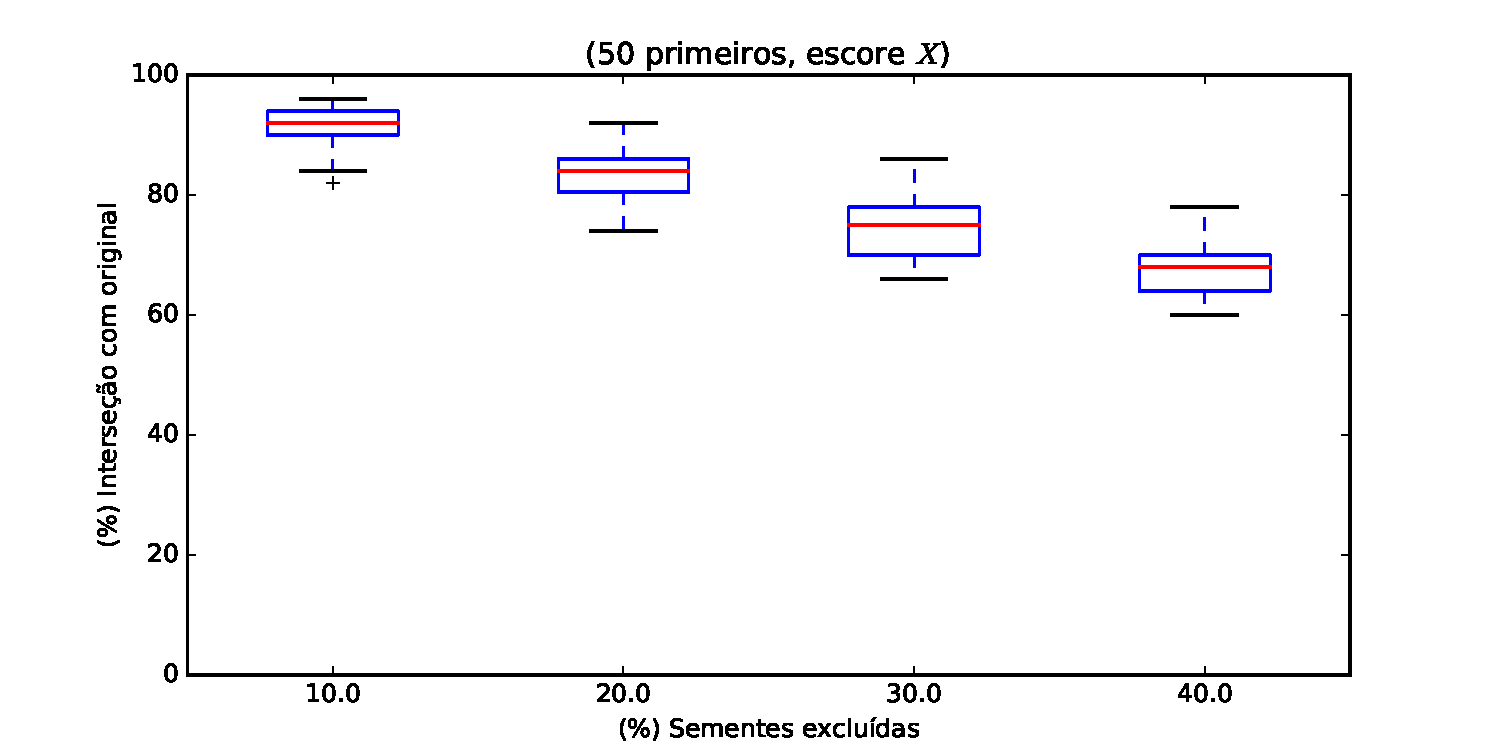
\includegraphics[width=1\textwidth]{Images/analyses/fig_X_50_40.pdf}
\caption {Análise dos 20 e 50 primeiros elementos ordenados por \textit{X}.
\label{fig_X_20-50_40}}
\flushleft{Fonte: Produzido pelos autores.}
\end{figure}
%

%
A Figura~\ref{fig_X_20-50_40} apresenta dois gráficos comparativos dos experimentos utilizando o método \textsl{Remoção de mais de um gene}, onde o gráfico de cima representa os \textsl{\textbf{20}} primeiros genes ranqueados pelos experimentos e o de baixo os primeiros \textsl{\textbf{50}}. Ambos no eixo \textsl{Horizontal} apresentam as porcentagens de genes sementes removidos em relação a amostra original e no eixo \textsl{Vertical}, a porcentagem de similaridade do resultado dos experimentos com o resultado original, ou seja, a similaridade das listas dos experimentos em relação a lista de ranqueamento gênico original.
%

Pode-se notar que, as amplitudes amostrais diminuíram em ambos os casos, isso demonstra uma menor variação dos experimentos em relação a análise feita dos \textsl{\textbf{10}} primeiros genes. Este comportamento, era intuitivamente esperado, em vista que ao aumentar a quantidade de genes selecionados na lista de ranqueamento, a probabilidade da variação dos resultados diminuírem aumenta. Porém, como são muitos genes na rede, o aumento de \textsl{\textbf{10}} e \textsl{\textbf{40}} genes ranqueados em relação a análise anterior, foi o suficiente para identificação. Apesar de ter sido esperado, representa um bom sinal de robustez, de modo que a baixa variação do resultado seja um fator para a mesma.
%

Nota-se também que no gráfico que representa os \textsl{\textbf{20}} primeiros genes ranqueados, quando analisou-se os experimentos que tiveram \textsl{\textbf{40\%}} dos genes sementes removidos em relação a amostra original, apresentaram experimentos \textsl{\textbf{ouliers}} onde alguns representavam uma boa correlação e outros uma má correlação. Isto indica que devemos observar os genes presentes nestes experimentos, para assim tentarmos entender o comportamento diferenciado. Os experimentos \textsl{\textbf{outliers}} que apresentaram uma má correlação, tiveram entre os seus genes sementes removidos os seguintes elementos \textsl{\textbf{TP53}} e \textsl{\textbf{RPGRIP1L}}. Estes genes sementes, são os que apresentaram um maior impacto em sua remoção única na etapa de \textsl{Remoção de um único gene}, onde podemos correlacionar que, o impacto mostra-se acumulativo, ou seja, se um gene com alto impacto em sua remoção é removido juntamente com outro gene causador de um alto impacto, ambos aumentam o impacto total da amostra em questão. Já os experimentos que apresentaram boa correlação, apresentaram a remoção de genes sementes que não causaram grande impacto em sua remoção na etapa de \textsl{Remoção de um único gene}, sendo exemplo destes os elementos \textsl{\textbf{GAD1}} e \textsl{\textbf{HP}}, estes que apresentaram um impacto sempre abaixo de \textsl{\textbf{10\%}}.   
%

Ao observar as medianas dos experimentos, pode-se enxergar que há uma diminuição conforme aumenta a quantidade de genes sementes removidos em relação ao experimento original. Este aspecto indica uma dependência do método NERI aos genes sementes, fato este já sabido previamente, devido ao mesmo valer-se destes genes para o ranqueamento gênico. O que chama a atenção é o fato da proporção de remoção ser menor que a proporção de impacto causado, ou seja, ao remover \textsl{\textbf{40\%}} dos genes sementes, não impacta o resultado em \textsl{\textbf{40\%}}, mas sim em menos, no caso dos \textsl{\textbf{20}} e \textsl{\textbf{50}} primeiros genes ranqueados, este impacto fica em torno dos \textsl{\textbf{35\%}}.



%
\subsubsection{Análise dos 100 e 200 primeiros elementos}
%
%Imagem
\begin{figure}[ht!]
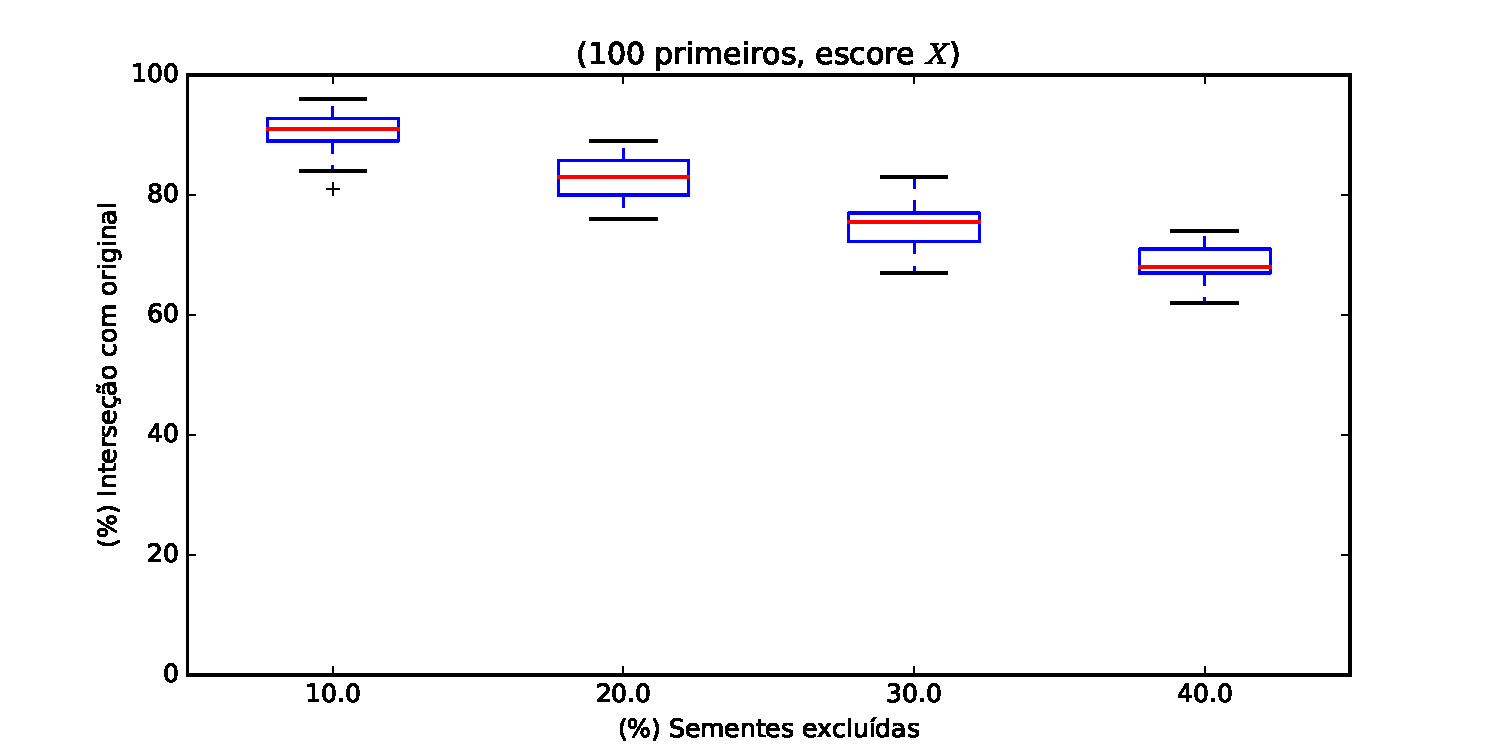
\includegraphics[width=1\textwidth]{Images/analyses/fig_X_100_40.pdf}
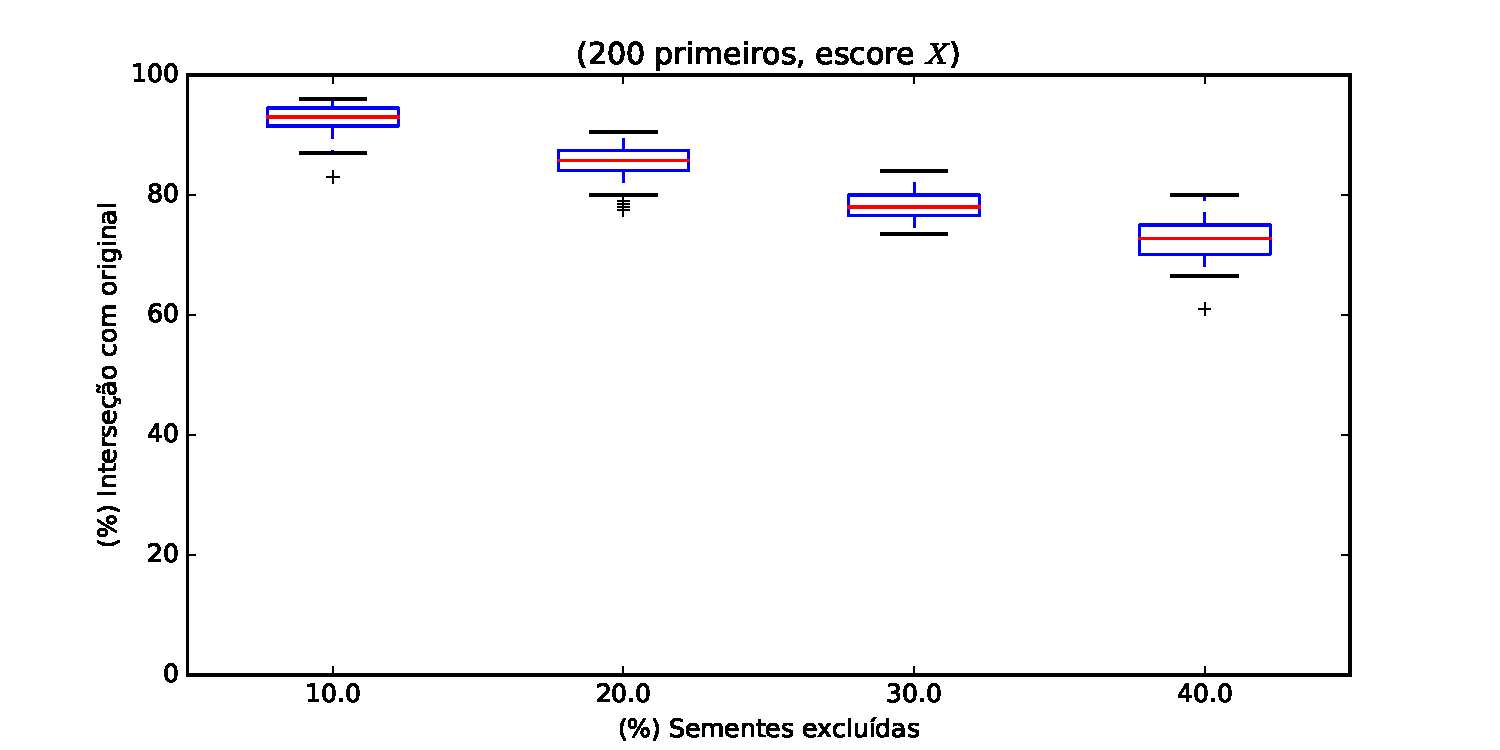
\includegraphics[width=1\textwidth]{Images/analyses/fig_X_200_40.pdf}
\caption {Análise dos 100 e 200 primeiros elementos ordenados por \textit{X}.
\label{fig_X_100-200_40}}
\flushleft{Fonte: Produzido pelos autores.}
\end{figure}
%%
%

%
A Figura~\ref{fig_X_100-200_40} apresenta dois gráficos comparativos em relação aos experimentos que foram gerados através do método \textsl{Remoção de mais de um gene}, onde o gráfico de cima representa os \textsl{\textbf{100}} primeiros genes ranqueados pelos experimentos e o de baixo os primeiros \textsl{\textbf{200}}. Ambos no eixo \textsl{Horizontal} apresentam as porcentagens de genes sementes removidos em relação a amostra original e no eixo \textsl{Vertical}, a porcentagem de similaridade do resultado dos experimentos com o resultado original, ou seja, a similaridade das listas dos experimentos em relação a lista de ranqueamento gênico original.
%

%
Podemos notar que mesmo os \textsl{outliers} presentes em ambos os gráficos apresentam uma boa correlação com o experimento original. Isto afirma que todos experimentos executados apresentaram um bom resultado de replicabilidade ao analisar os primeiros \textbf{\textsl{100}} e \textbf{\textsl{200}} genes priorizados pelo método NERI. Este aspecto indica uma forte robustez do método, em vista que mesmo os experimentos que apresentaram comportamento diferente do conjunto no qual estão inseridos obtiveram uma boa correlação com o experimento original.

%
Outro aspecto importante para se observar é o comportamento das correlações dos experimentos, quanto maior a quantidade de genes sementes removidos da amostra original, menor a correlação obtida com o experimento original. Este comportamento esteve presente em todas as análises feitas, tanto no escore $X$ quanto no $\Delta'$, comprovando a dependência do método NERI em relação aos genes sementes. Porém mesmo assim, apresentou-se robusto a remoção dos genes sementes, indicando bons resultados de replicabilidade. Fato este que torna a utilização do método analisado mais confiável. 
%

%
\subsection{
\label{sec:compXS}
Comparação do escore $X$ com o escore $\Delta'$}
%

Podemos notar que o escore $X$ é mais robusto em relação a remoção de genes sementes se comparado com o escore $\Delta'$, apresentando menor variação nos resultados e um menor impacto no resultado final em relação a amostra original. Um fator impactante é a comparação das Figuras~\ref{fig_X_10_40} (\textsl{\textbf{10}} primeiros genes ordenados pelo score $X$) e \ref{fig_S_10_40} (\textsl{\textbf{10}} primeiros genes ordenados pelo score $\Delta'$), onde podemos observar a diferença das correlações nos \textsl{boxplots} referentes a \textsl{\textbf{40\%}} de remoção dos genes sementes em relação a amostra original. O \textsl{boxplot} que representa a ordenação pelo score $\Delta'$ apresenta uma amplitude amostral onde o valor mínimo representado é de aproximadamente \textsl{\textbf{10\%}} de similaridade com a amostra original, valor este que apresenta-se muito baixo se comparado com o \textsl{boxplot} que representa a ordenação pelo score $X$ onde o valor mínimo apresentado é por um experimento com comportamento \textsl{outlier} e corresponde a \textsl{\textbf{40\%}} de similaridade com a amostra original. Outra métrica observada é a amplitude amostral de ambos, ainda observando o pior caso (\textsl{\textbf{40\%}} de remoção dos genes sementes em relação a amostra original), onde o score $X$ apresenta \textsl{\textbf{30\%}} de variação contra \textsl{\textbf{80\%}} apresentado pelo score $\Delta'$.
%

%
As variações dos resultados e a amplitude interquartílica dos \textsl{boxplots} apresentam-se maiores em $\Delta'$ em todas as análises comparativas entre aos dois escores. Isto indica novamente uma maior confiabilidade em termos de variação de resultado no score $X$. Este comportamento se dá pela natureza dos scores, onde o score $X$ é baseado na soma de todas as medidas de centralidade calculadas pelo método NERI e o score $\Delta'$ é baseado nas pontuações condicionais da rede, fato este que ao faltar um determinado gene semente que representaria algum papel na rede, o score condicional apresenta variação. Sendo assim, uma forma de ranqueamento gênico menos confiável que o embasamento no score $X$. Este fato não invalida a utilização da mesma, em vista que esta apresentou bons resultados em linhas gerais, onde o impacto no resultado final em pouquíssimos casos ficou acima de \textsl{\textbf{50\%}} (em casos de extremo estresse, como na remoção de \textsl{\textbf{40\%}} dos genes sementes em relação a amostra original e observando o apenas os \textsl{\textbf{10}} primeiros genes ranqueados).
%

\section{Desempenho computacional}
%\textcolor{red}{======= REESCREVER DAQUI P BAIXO =======}

%Podemos considerar que o método tende a ser robusto ao observar os top 10 primeiros genes selecionados, levando em conta seu comportamento em relação a remoção de genes sementes do experimento, porém ainda não podemos tirar conclusões concretas sem antes observar sob outras perspectivas os resultados dos experimentos, como por exemplo, o espalhamento dos resultados em relação ao eixo Y de cada agrupamento, existem amostras que apresentaram resultados muito discrepantes em relação ao conjunto no qual ele pertence.
%Para estudar estes casos, alguns aspectos devem ser analisados, sendo um deles, quais genes foram removidos e quais não foram, isso permitirá um melhor entendimento do comportamento dos \textsl{outliers}.



Os fatores envolvidos no processo de execução dos experimentos, foram as configurações da máquina no qual foi executada e a disponibilidade de tempo execução.
As configurações da maquina no qual foram executados os experimentos são as descritas abaixo:

\begin{itemize}
    \item \textbf{Processador:} \textsl{i7} geração 5.
    \item \textbf{Memória:} 16 GB - 2 pentes 8GB DDR3 1600Ghz.
    \item \textbf{Armazenamento:} 50 GB HD disponíveis.
\end{itemize}

 
Pelo fato do programa que implementa o método NERI ainda não utilizar paralelismo (utilização de mais de um núcleo de processamento), foram executadas 4 instâncias separadas ao mesmo tempo, durante todo a etapa de execução do experimento.

\subsection{Consumo de Processamento}
Cada instância ocupou 100\% de processamento de um núcleo físico presente no processador, como a máquina utilizada possui 4 núcleos físicos e foram executadas 4 instâncias simultaneamente, o consumo de cpu foi para 100\% do total presente.

\subsection{Consumo de Memória}
Cada instância em execução consumiu em média 1,5 GB de memória, totalizando aproximadamente 6 GB alocados por todas as 4 instâncias executantes.

\subsection{Utilização de disco}
Devido ao fato de os experimentos serem executados em modo \textsl{Debug}, a escrita em arquivo dos \textsl{logs} foi realizada durante boa parte do tempo de execução.
Isto significa que, se os modo \textsl{Debug} for desabilitado, os tempos podem ser um pouco menores.
Os 30 experimentos ocuparam aproximadamente 6,5 MB; para a remoção de um único gene foram realizados 30 experimentos (um para cada semente); e para a remoção de vários genes foram realizados 50 experimentos para cada percentual de remoção (10\%, 20\%, 30\% e 40\%), totalizando $50 x 4 = 200$ experimentos de remoção de vários genes.
Desta forma, os 230 experimentos realizados ocuparam aproximadamente 1,2 GB de armazenamento no disco rígido.


% ----------------------------------------------------------
% Finaliza a parte no bookmark do PDF
% para que se inicie o bookmark na raiz
% e adiciona espaço de parte no Sumário
% ----------------------------------------------------------
\phantompart

% ---
% Conclusão
% ---
\chapter[Considerações Finais]{Considerações Finais}

\section{Trabalhos Futuros}

\begin{enumerate}
\item a
    \item b
    \item c
\end{enumerate}

% ---



% ----------------------------------------------------------
% ELEMENTOS PÓS-TEXTUAIS
% ----------------------------------------------------------
\postextual
% ----------------------------------------------------------

% ----------------------------------------------------------
% Referências bibliográficas
% ----------------------------------------------------------
\bibliography{abntex2-modelo-references}

% ----------------------------------------------------------
% Glossário
% ----------------------------------------------------------
%
% Consulte o manual da classe abntex2 para orientações sobre o glossário.
%
%\glossary


% ----------------------------------------------------------
% Apêndices
% ----------------------------------------------------------

% ---
% Inicia os apêndices
% ---

\begin{apendicesenv}

%\renewcommand{\appendixtocname}{Apêndices}
%\renewcommand{\appendixpagename}{Apêndices}




% Imprime uma página indicando o início dos apêndices
%\partapendices


\captionsbrazil
\chapter{Tabelas}
\label{appendice_tables}

% ======= Tabela de genes sementes ==========
\begin{table}[]
\centering
\tiny
\caption{Tabela com os genes sementes do experimento original}
\label{table_original_seeds}
\begin{tabular}{@{}rlll@{}}
\toprule
\textbf{\textsl{Code 1}} & \textbf{GENE} &   \textbf{Description} & \textbf{Code 2} \\ \midrule
4524 & \textbf{MTHFR} & 5,10-methylenetetrahydrofolate reductase (NADPH) & 1p36.3 \\
5999 & \textbf{RGS4} & regulator of G-protein signaling 4 & 1q23.3 \\
5362 & \textbf{PLXNA2} & plexin A2 & 1q32.2 \\
27185 & \textbf{DISC1} & disrupted in schizophrenia 1 & 1q42.1 \\
7166 & \textbf{TPH1} & tryptophan hydroxylase 1 & 11p15.3-p14 \\
1815 & \textbf{DRD4} & dopamine receptor D4 & 11p15.5 \\
2900 & \textbf{GRIK4} & glutamate receptor, ionotropic, kainate 4 & 11q22.3 \\
1813 & \textbf{DRD2} & dopamine receptor D2 & 11q23 \\
9638 & \textbf{FEZ1} & fasciculation and elongation protein zeta 1 (zygin I) & 11q24.2 \\
4978 & \textbf{OPCML} & opioid binding protein/cell adhesion molecule-like & 11q25 \\
2904 & \textbf{GRIN2B} & glutamate receptor, ionotropic, N-methyl D-aspartate 2B & 12p12 \\
1610 & \textbf{DAO} & D-amino-acid oxidase & 12q24 \\
3356 & \textbf{HTR2A} & 5-hydroxytryptamine (serotonin) receptor 2A & 13q14-q21 \\
207 & \textbf{AKT1} & v-akt murine thymoma viral oncogene homolog 1 & 14q32.32|14q32.32 \\
23322 & \textbf{RPGRIP1L} & RPGRIP1-like & 16q12.2 \\
3240 & \textbf{HP} & haptoglobin & 16q22.1 \\
7157 & \textbf{TP53} & tumor protein p53 & 17p13.1 \\
6532 & \textbf{SLC6A4} & solute carrier family 6, member 4 & 17q11.1-q12 \\
348 & \textbf{APOE} & apolipoprotein E & 19q13.2 \\
3553 & \textbf{IL1B} & interleukin 1, beta & 2q14 \\
2571 & \textbf{GAD1} & glutamate decarboxylase 1 (brain, 67kDa) & 2q31 \\
91752 & \textbf{ZNF804A} & zinc finger protein 804A & 2q32.1 \\
2066 & \textbf{ERBB4} & v-erb-a erythroblastic leukemia viral oncogene homolog 4 & 2q33.3-q34 \\
1312 & \textbf{COMT} & catechol-O-methyltransferase & 22q11.21-q11.23|22q11.21 \\
2561 & \textbf{GABRB2} & gamma-aminobutyric acid (GABA) A receptor, beta 2 & 5q34 \\
1812 & \textbf{DRD1} & dopamine receptor D1 & 5q35.1 \\
2913 & \textbf{GRM3} & glutamate receptor, metabotropic 3 & 7q21.1-q21.2 \\
5649 & \textbf{RELN} & reelin & 7q22 \\
3084 & \textbf{NRG1} & neuregulin 1 & 8p12 \\
5533 & \textbf{PPP3CC} & protein phosphatase 3 (formerly 2B), catalytic subunit & 8p21.3 \\
267012 & *DAOA & D-amino acid oxidase activator & 13q33.2|13q34 \\
64067 & *NPAS3 & neuronal PAS domain protein 3 & 14q12-q13 \\
1139 & *CHRNA7 & cholinergic receptor, nicotinic, alpha 7 & 15q14 \\
5625 & *PRODH & proline dehydrogenase (oxidase) 1 & 22q11.21 \\
84062 & *DTNBP1 & dystrobrevin binding protein 1 & 6p22.3 \\
266553 & *OFCC1 & orofacial cleft 1 candidate 1 & 6p24.3 \\
63915 & *MUTED & muted homolog (mouse) & 6p25.1-p24.3 \\
6570 & *SLC18A1 & solute carrier family 18 (vesicular monoamine), member 1 & 8p21.3 \\ \bottomrule
\end{tabular}

\flushleft{Obs: durante a integração, apenas os 30 primeiros genes sementes possuíam correspondentes na rede \textsl{\textbf{PPI}}. Os 8 últimos genes (com o marcador \textsl{\textbf{*}})  não apresentaram integração com a rede \textsl{\textbf{PPI}}.

Fonte: Tabela gerada pelo autor.}
\end{table}

% ===========================================


% ========================== APENDICE SCRIPTS ======================

\chapter{Scripts}
\label{appendice_scripts}

\tiny
\label{CVV_script}
\begin{lstlisting}[caption={Script em Python para geração dos experimentos com remoção de mais de um gene semente.},label=getBlockStatic,language=Python]

class CrossValidationBased():
	def __init__(self):
		self.LEntrada = []  #Ex: [1,2,4,5,6]
		self.lenEntrada = 0 #Tamanho entrada
		self.LSaida = []    #Lista de saida
		self.k = 0          #iteracoes
		self.remocoes = 0   #Qtd Remocoes
		self.newLen = 0 
		self.removidas = []


	''' 
	 @params list {[]}	(Lista semente)
	 @params rem {int}	(% da lista a ser removida)
	 @params it {int}	(quantidade de listas a serem geradas)
	 ''' 
	def setData(self,list,rem,it):
		self.LEntrada = list
		self.k = it
		self.lenEntrada = len(self.LEntrada)
		self.remocoes = int(rem*self.lenEntrada)
		self.newLen = self.lenEntrada - self.remocoes
		self.result = []
		self.removidas = []
		
	def generateResult(self):
		self.result = []
		self.removidas = []
		while(self.k>0):
			self.LSaida = []
			LNRemovidas = self.LEntrada[:]
			novoLen = self.lenEntrada
			while(novoLen > self.remocoes):
				r = random.randrange(0,novoLen)
				self.LSaida.append(LNRemovidas[r])
				LNRemovidas.pop(r)
				novoLen -= 1

			self.result.append(self.LSaida)
			self.removidas.append(LNRemovidas)
			self.k -=1

    '''
    Retorna lista de conjuntos resultantes
    @returns self.result {[[]]}
    '''
	def getResult(self):
		return self.result

    '''
    Retorna lista de conjuntos removidos em cada agrupamento
    @returns self.removidas {[]}
    '''
	def getRemovidas(self):
		return self.removidas


\end{lstlisting}



\tiny
\label{shell_run_all}
\begin{lstlisting}[caption={Script em \textsl{Shell} para execução automatizada dos experimentos.},label=getBlockStatic,language=Shell]
#! /bin/bash
program="neri.py"
call_command="python"
params="--nodisplay run"
temp_archive_map="mapIn.txt"
processed="processed.txt"

while read line; do
	 $call_command $program $params $line
	echo $line >> $processed
done < $temp_archive_map

\end{lstlisting}



\chapter{Configuração do ambiente}
\label{appendice_ambient}

%Imagem - Arvore de arquivos
\begin{figure}[ht!]
\centering
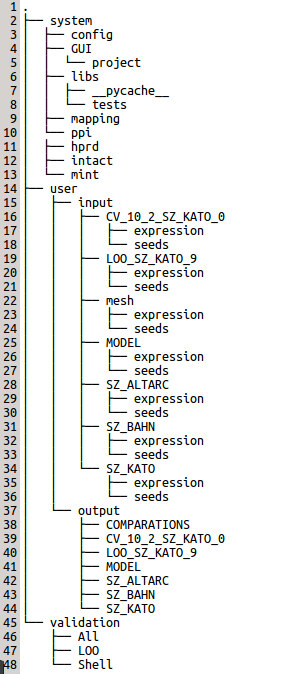
\includegraphics[width=80mm]{Images/tree.png}
\caption {Árvore de arquivos do programa \textsl{NERI}
\label{tree_files}}
\flushleft{
Árvore de arquivos 

Fonte: Produzido pelos autores.}
\end{figure}





\end{apendicesenv}
% ---
\begin{comment}

% ----------------------------------------------------------
% Anexos
% ----------------------------------------------------------

% ---
% Inicia os anexos
% ---
\begin{anexosenv}

% Imprime uma página indicando o início dos anexos
\partanexos

% ---
\chapter{Morbi ultrices rutrum lorem.}
% ---
\lipsum[30]

% ---
\chapter{Cras non urna sed feugiat cum sociis natoque penatibus et magnis dis
parturient montes nascetur ridiculus mus}
% ---

\lipsum[31]

% ---
\chapter{Fusce facilisis lacinia dui}
% ---

\lipsum[32]

\end{anexosenv}
\end{comment}
%---------------------------------------------------------------------
% INDICE REMISSIVO
%---------------------------------------------------------------------
\phantompart

%---------------------------------------------------------------------

\end{document}